%
% ---------------------------------------------------------------
% Copyright (C) 2012-2018 Gang Li
% ---------------------------------------------------------------
%
% This work is the default powerdot-tuliplab style test file and may be
% distributed and/or modified under the conditions of the LaTeX Project Public
% License, either version 1.3 of this license or (at your option) any later
% version. The latest version of this license is in
% http://www.latex-project.org/lppl.txt and version 1.3 or later is part of all
% distributions of LaTeX version 2003/12/01 or later.
%
% This work has the LPPL maintenance status "maintained".
%
% This Current Maintainer of this work is Gang Li.
%
%

\documentclass[
 size=14pt,
 paper=smartboard,  %a4paper, smartboard, screen
 mode=present, 		%present, handout, print
 display=slides, 	% slidesnotes, notes, slides
 style=tuliplab,  	% TULIP Lab style
 pauseslide,
 fleqn,leqno]{powerdot}


\usepackage{cancel}
\usepackage{caption}
\usepackage{stackengine}
\usepackage{smartdiagram}
\usepackage{attrib}
\usepackage{amssymb}
\usepackage{amsmath} 
\usepackage{amsthm} 
\usepackage{mathtools}
\usepackage{rotating}
\usepackage{graphicx}
\usepackage{boxedminipage}
\usepackage{rotate}
\usepackage{calc}
\usepackage[absolute]{textpos}
\usepackage{psfrag,overpic}
\usepackage{fouriernc}
\usepackage{pstricks,pst-3d,pst-grad,pstricks-add,pst-text,pst-node,pst-tree}
\usepackage{moreverb,epsfig,subfigure}
\usepackage{color}
\usepackage{booktabs}
\usepackage{etex}
\usepackage{breqn}
\usepackage{multirow}
\usepackage{natbib}
\usepackage{bibentry}
\usepackage{gitinfo2}
\usepackage{siunitx}
\usepackage{nicefrac}
%\usepackage{geometry}
%\geometry{verbose,letterpaper}
\usepackage{media9}
\usepackage{animate}
%\usepackage{movie15}
\usepackage{auto-pst-pdf}

\usepackage{breakurl}
\usepackage{fontawesome}
\usepackage{xcolor}
\usepackage{multicol}



\usepackage{verbatim}
\usepackage[utf8]{inputenc}
\usepackage{dtk-logos}
\usepackage{tikz}
\usepackage{adigraph}
%\usepackage{tkz-graph}
\usepackage{hyperref}
%\usepackage{ulem}
\usepackage{pgfplots}
\usepackage{verbatim}
\usepackage{fontawesome}


\usepackage{todonotes}
% \usepackage{pst-rel-points}
\usepackage{animate}
\usepackage{fontawesome}

\usepackage{listings}
\lstset{frameround=fttt,
frame=trBL,
stringstyle=\ttfamily,
backgroundcolor=\color{yellow!20},
basicstyle=\footnotesize\ttfamily}
\lstnewenvironment{code}{
\lstset{frame=single,escapeinside=`',
backgroundcolor=\color{yellow!20},
basicstyle=\footnotesize\ttfamily}
}{}


\usepackage{hyperref}
\hypersetup{ % TODO: PDF meta Data
  pdftitle={Presentation Title},
  pdfauthor={Gang Li},
  pdfpagemode={FullScreen},
  pdfborder={0 0 0}
}


% \usepackage{auto-pst-pdf}
% package to show source code

\definecolor{LightGray}{rgb}{0.9,0.9,0.9}
\newlength{\pixel}\setlength\pixel{0.000714285714\slidewidth}
\setlength{\TPHorizModule}{\slidewidth}
\setlength{\TPVertModule}{\slideheight}
\newcommand\highlight[1]{\fbox{#1}}
\newcommand\icite[1]{{\footnotesize [#1]}}

\newcommand\twotonebox[2]{\fcolorbox{pdcolor2}{pdcolor2}
{#1\vphantom{#2}}\fcolorbox{pdcolor2}{white}{#2\vphantom{#1}}}
\newcommand\twotoneboxo[2]{\fcolorbox{pdcolor2}{pdcolor2}
{#1}\fcolorbox{pdcolor2}{white}{#2}}
\newcommand\vpspace[1]{\vphantom{\vspace{#1}}}
\newcommand\hpspace[1]{\hphantom{\hspace{#1}}}
\newcommand\COMMENT[1]{}

\newcommand\placepos[3]{\hbox to\z@{\kern#1
        \raisebox{-#2}[\z@][\z@]{#3}\hss}\ignorespaces}

\renewcommand{\baselinestretch}{1.2}


\newcommand{\draftnote}[3]{
	\todo[author=#2,color=#1!30,size=\footnotesize]{\textsf{#3}}	}
% TODO: add yourself here:
%
\newcommand{\gangli}[1]{\draftnote{blue}{GLi:}{#1}}
\newcommand{\shaoni}[1]{\draftnote{green}{sn:}{#1}}
\newcommand{\gliMarker}
	{\todo[author=GLi,size=\tiny,inline,color=blue!40]
	{Gang Li has worked up to here.}}
\newcommand{\snMarker}
	{\todo[author=Sn,size=\tiny,inline,color=green!40]
	{Shaoni has worked up to here.}}

%%%%%%%%%%%%%%%%%%%%%%%%%%%%%%%%%%%%%%%%%%%%%%%%%%%%%%%%%%%%%%%%%%%%%%%%
% title
% TODO: Customize to your Own Title, Name, Address
%
\title{Sentiment Analysis On Movie Reviews}
\author{
MingZhu Kang 
\\
\\Xi'an Shiyou University
%\\Deakin University
\\Chinese Academy of Sciences
%\\ \today
}
%\date{\gitCommitterDate}


% Customize the setting of slides
\pdsetup{
% TODO: Customize the left footer, and right footer
rf=\href{http://www.tulip.org.au}{
Last Changed by: \textsc{\gitCommitterName}\ (\gitAuthorDate)
%Last Changed by: \textsc{\gitCommitterName}\ \gitVtagn-\gitAbbrevHash\ (\gitAuthorDate)
},
cf={Sentiment Analysis On Movie Reviews},
}


\begin{document}

\maketitle

%\begin{slide}{Overview}
%\tableofcontents[content=sections]
%\end{slide}


%%==========================================================================================
%%
% \begin{slide}[toc=,bm=]{Overview}
% \tableofcontents[content=currentsection,type=1]
% \end{slide}
%%
%%==========================================================================================


\section{Introduction}


%%==========================================================================================
%%
\begin{slide}{Project  Introduction}
\begin{center}
\twotonebox{\rotatebox{95}{Defn}}{\parbox{.89\textwidth}
{
\begin{itemize}
\item Project Introduction
\\ This competition presents a chance to benchmark your sentiment-analysis ideas 
on the Rotten Tomatoes dataset. 
You are asked to label phrases on a scale of five values: negative, somewhat negative, neutral, somewhat positive, 
positive. Obstacles like sentence negation, sarcasm, terseness, language ambiguity.
The Rotten Tomatoes movie review dataset is a corpus of movie reviews used for sentiment analysis, 
This project needs to classify the sentiment of sentences from the Rotten Tomatoes dataset.
\end{itemize}
}}

\end{center}
\bigskip
\begin{center}
\begin{tabular}{c| c c c c }
\toprule
\midrule

\bottomrule
\end{tabular}
\end{center}
\bigskip

%%==========================================================================================
\begin{note}
First, I will introduce the problem definition.
In the real life,
a teacher may be interested in the characteristics that
make one student obvious different from others.
Or,
NBA sports coaches would prefer to
know the advantages and disadvantages of one player.
Here, the player can be regarded as a query object.

For example, team A has five players,
each player has four features.
The NBA sports coaches may want to know the features of
player $1$ that are different from others.

The above example can be seen as outlying aspects mining.
The main purpose of outlying aspects mining is to identify
the outstanding features of the query object.
\end{note}
%%==========================================================================================

\end{slide}
%%
%%==========================================================================================


%%
%%==========================================================================================


\section{Import Data Set}


%%==========================================================================================
%%
\begin{slide}{Preprocessing Of Project Data Sets}
%Related Work - Outlying Aspects Mining
\begin{itemize}
  \item Data Collection 
  \\Download dataset from the kaggle project.
  \\train.tsv contains the phrases and their associated sentiment labels. 
\\Official website also have additionally provided a SentenceId 
so that you can track which phrases belong to a single sentence.
\end{itemize}
  \begin{figure}[htbp]
    \centering
    \begin{minipage}[t]{0.58\textwidth}
      \centering
      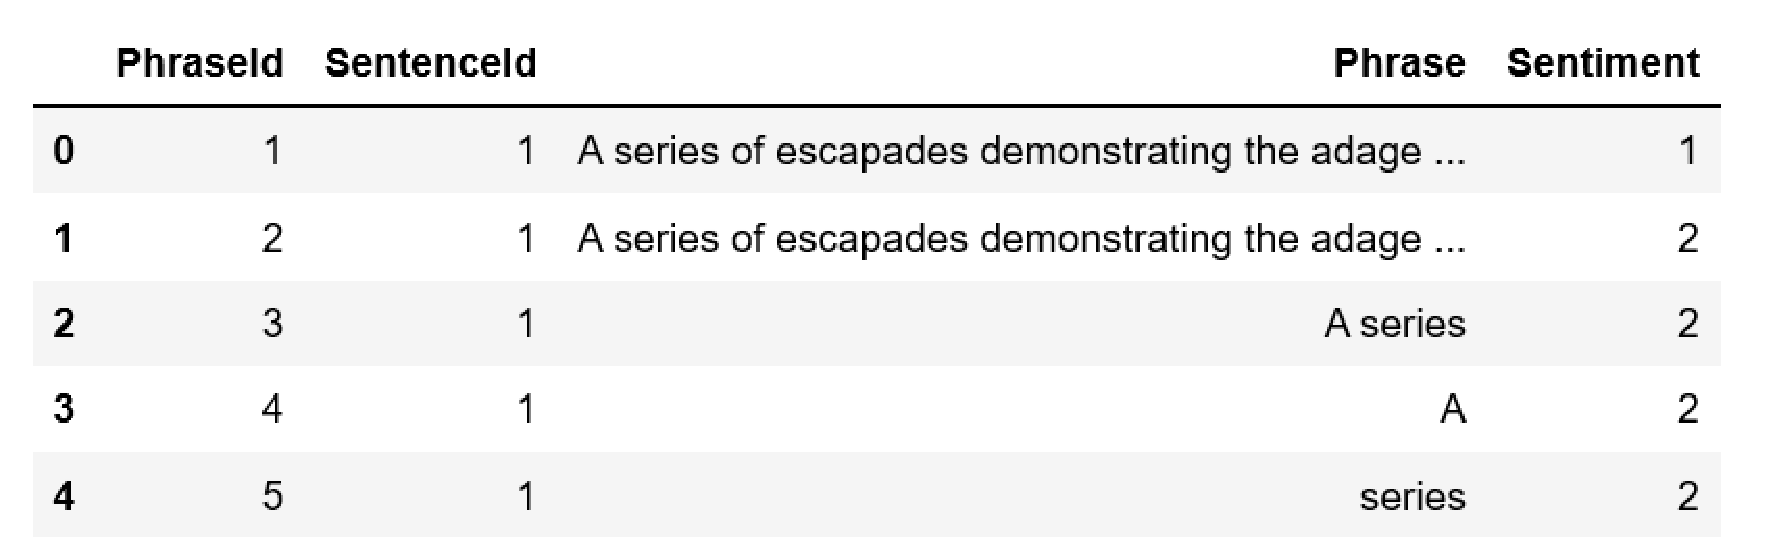
\includegraphics[width=1.2\textwidth]{logos/train.eps}
      \vspace{0.4em}
      %\caption{Download dataset display from kaggle}
    \end{minipage}
  \end{figure}
\bigskip





%%==========================================================================================
\begin{note}
Let me introduce two existing methods:
Feature selection and score-and-search.

For feature selection,
the query point can be regarded as positive class and
the rest of the data can be regarded as negative class,
selected the features that best distinguish the two classes.

The advantages of this method are easy to operate,
and it's able to resolve dimensionality bias.
However, it has some drawbacks.
Firstly,
positive and negative classes are Not balanced,
secondly,
it can't quantify the outlying degree correctly.
Most importantly,
it doesn't identify group outlying aspects.
\end{note}
%%==========================================================================================

\end{slide}
%%
%%==========================================================================================

%%
%%==========================================================================================
% \begin{slide}{Feature Item}
% By making a comprehensive analysis of the nine
% characteristic items in the data set mentioned 
% above,we can reach the following conclusions:


% \bigskip

% \begin{figure}[htbp]
%   \centering
%   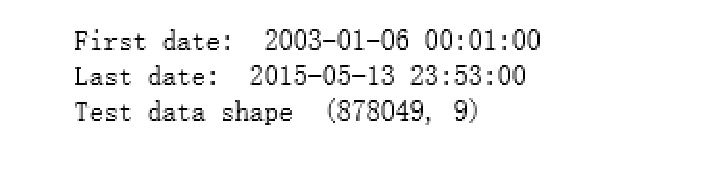
\includegraphics[width=1\textwidth]{kaggle/1.eps}
%   \caption{}
% \end{figure}
% \setlength{\parindent}{2em}The data range was from 1/1/2003 to 5/13/2015, and 
% a data training set containing nine feature items and 87,8049 
% samples was created.
% \end{slide}

%%
%%==========================================================================================
% \begin{slide}{Features Item}
%   \begin{figure}
%     \centering
%     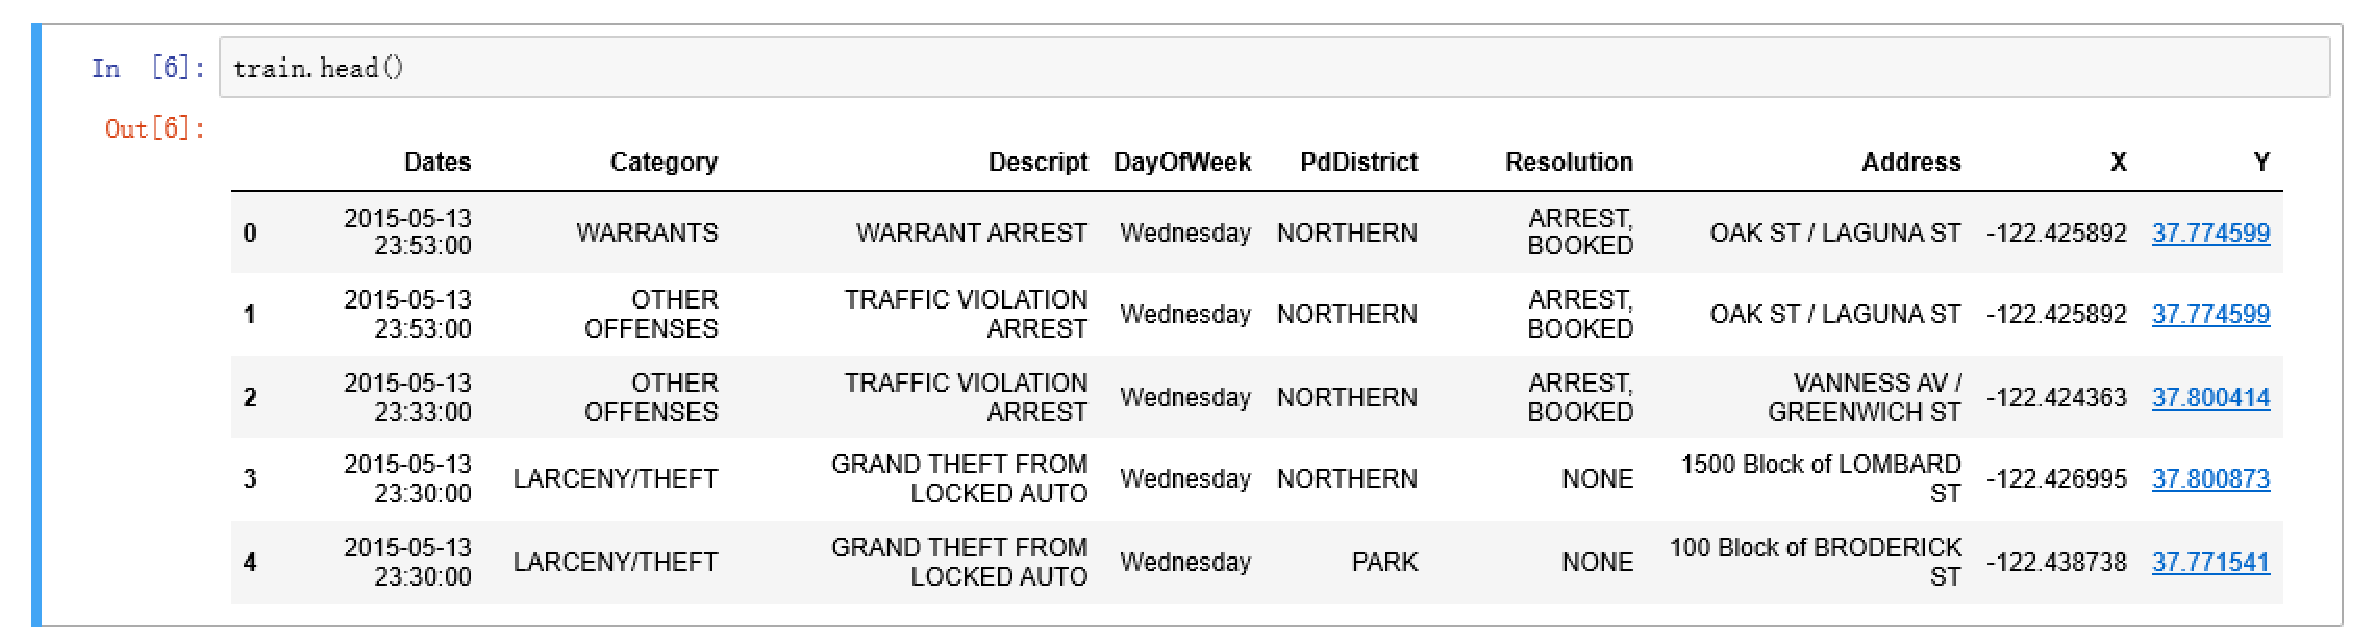
\includegraphics[width=1\textwidth]{kaggle/2.eps}
%   \end{figure}
  
%   \bigskip
% More specifically it includes the following variables.
%   \begin{itemize}
%     \item Date - timestamp of the crime Incident.
%     \item Category - category of the crime incident. (This is our target variable.)
%     \item Descript - detailed description of the crime incident
%     \item DayOfWeek - the day of the week
%     \item PdDistrict - the name of the Police Department District
%     \item Resolution - The resolution of the crime incident

%   \end{itemize}
% \end{slide}
%%
%%==================================================================



% \begin{slide}{Features Item}
%   \begin{itemize}
%     \item Address - the approximate street address of the crime incident
%     \item X - Longitude
%     \item Y - Latitude
%   \end{itemize}
% \end{slide}

%%==========================================================================================
\begin{slide}{Preprocessing Of Project Data Sets}
  %Related Work - Outlying Aspects Mining
  \begin{itemize}
    \item Data Collection 
    \\test.tsv contains just phrases. You must assign a sentiment label to each phrase.
  \end{itemize}
    \begin{figure}[htbp]
      \centering
      \begin{minipage}[t]{0.58\textwidth}
        \centering
        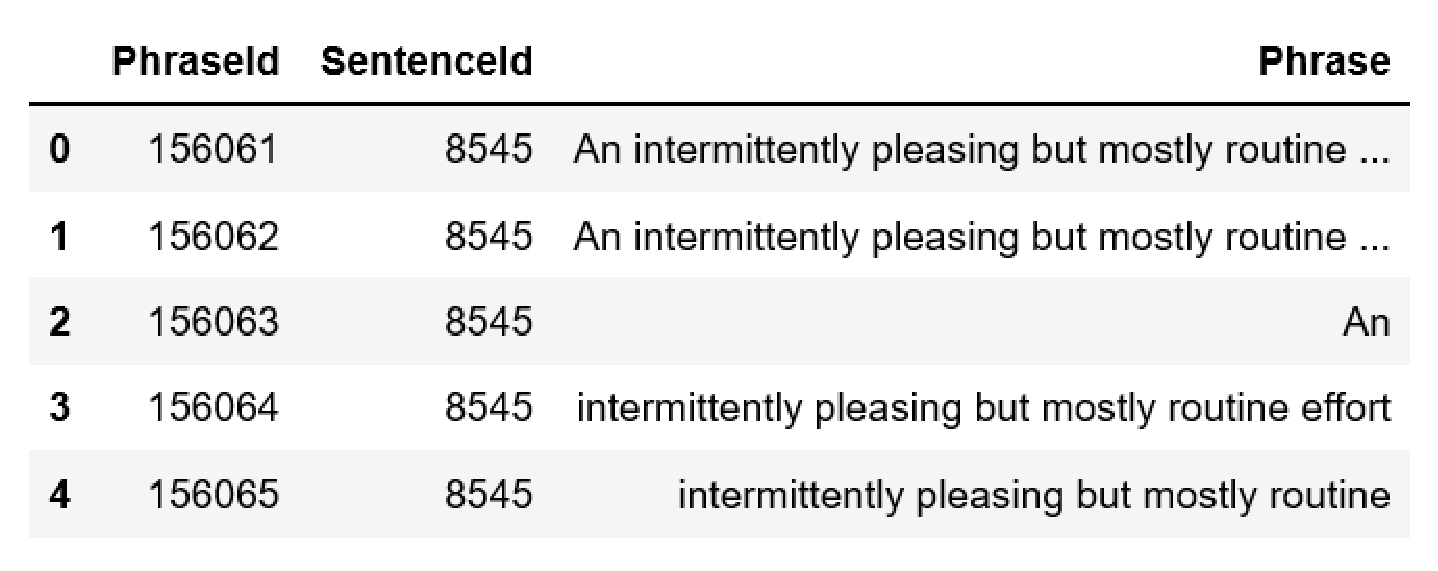
\includegraphics[width=1.2\textwidth]{logos/test.eps}
        \vspace{0.4em}
        %\caption{Download dataset display from kaggle}
      \end{minipage}
    \end{figure}
  \bigskip
\end{slide}

\section{Build A Corpus}

%%==========================================================================================
%%

%%
%%===========================================================================================



%%
%%=============================================================================================
\begin{slide}[toc=,bm=]{Build A Corpus}
\begin{itemize}
\item 
To extract the text contents of the training set and the test set, 
a corpus was constructed,and the text contents of the training set 
and the test set were combined together to extract the emotional tags 
of the training set through concat function.
\end{itemize}
\begin{figure}[htbp]
  \centering
  \begin{minipage}[t]{0.48\textwidth}
    \centering
    \centerline{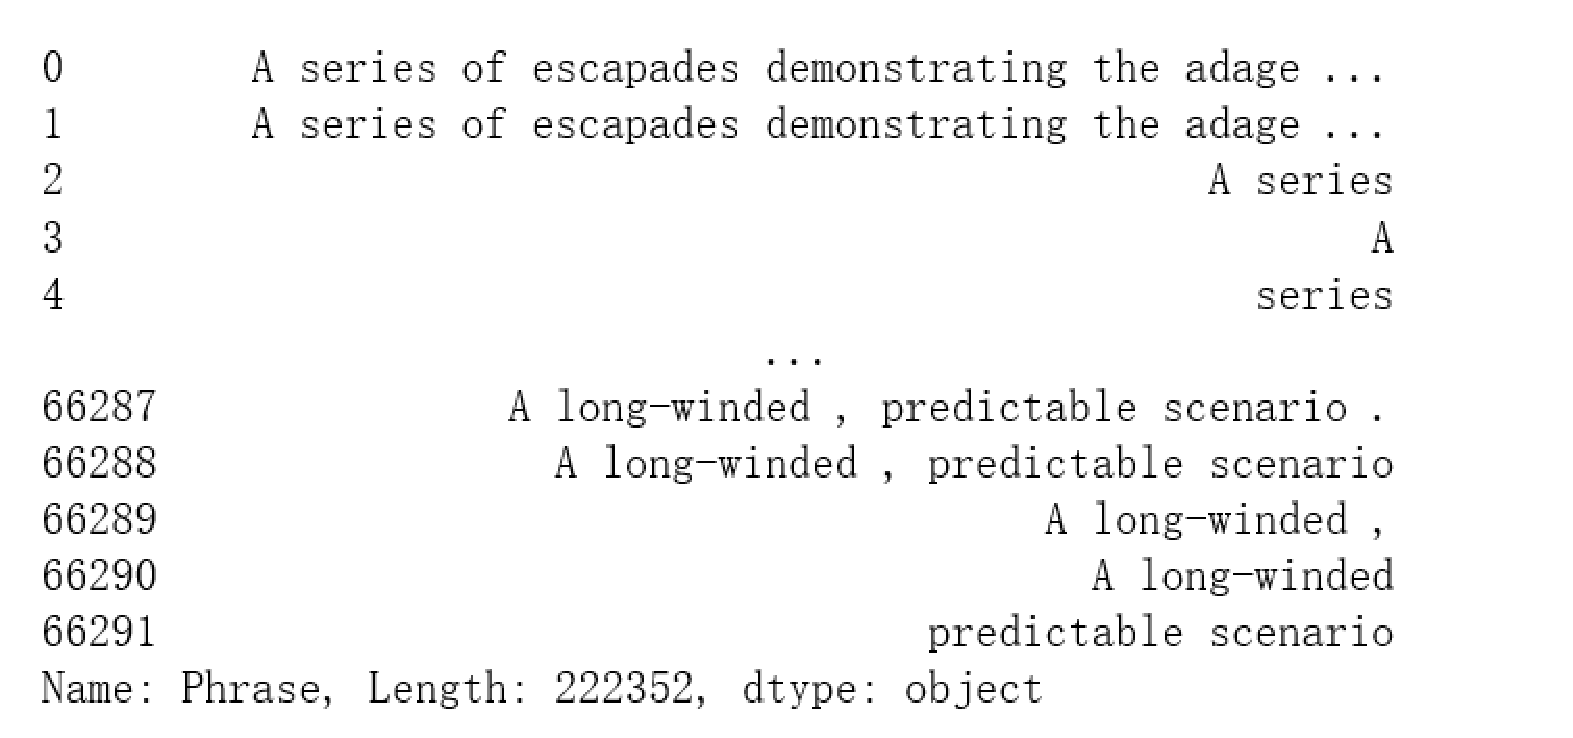
\includegraphics[width=1.5\textwidth]{logos/hebing.eps}}
    \vspace{0.4em}
    %\caption{Download dataset display from kaggle}
  \end{minipage}
\end{figure}


% \begin{figure}[htbp]
%   \centering
%   \begin{minipage}[t]{0.48\textwidth}
%     \centering
%     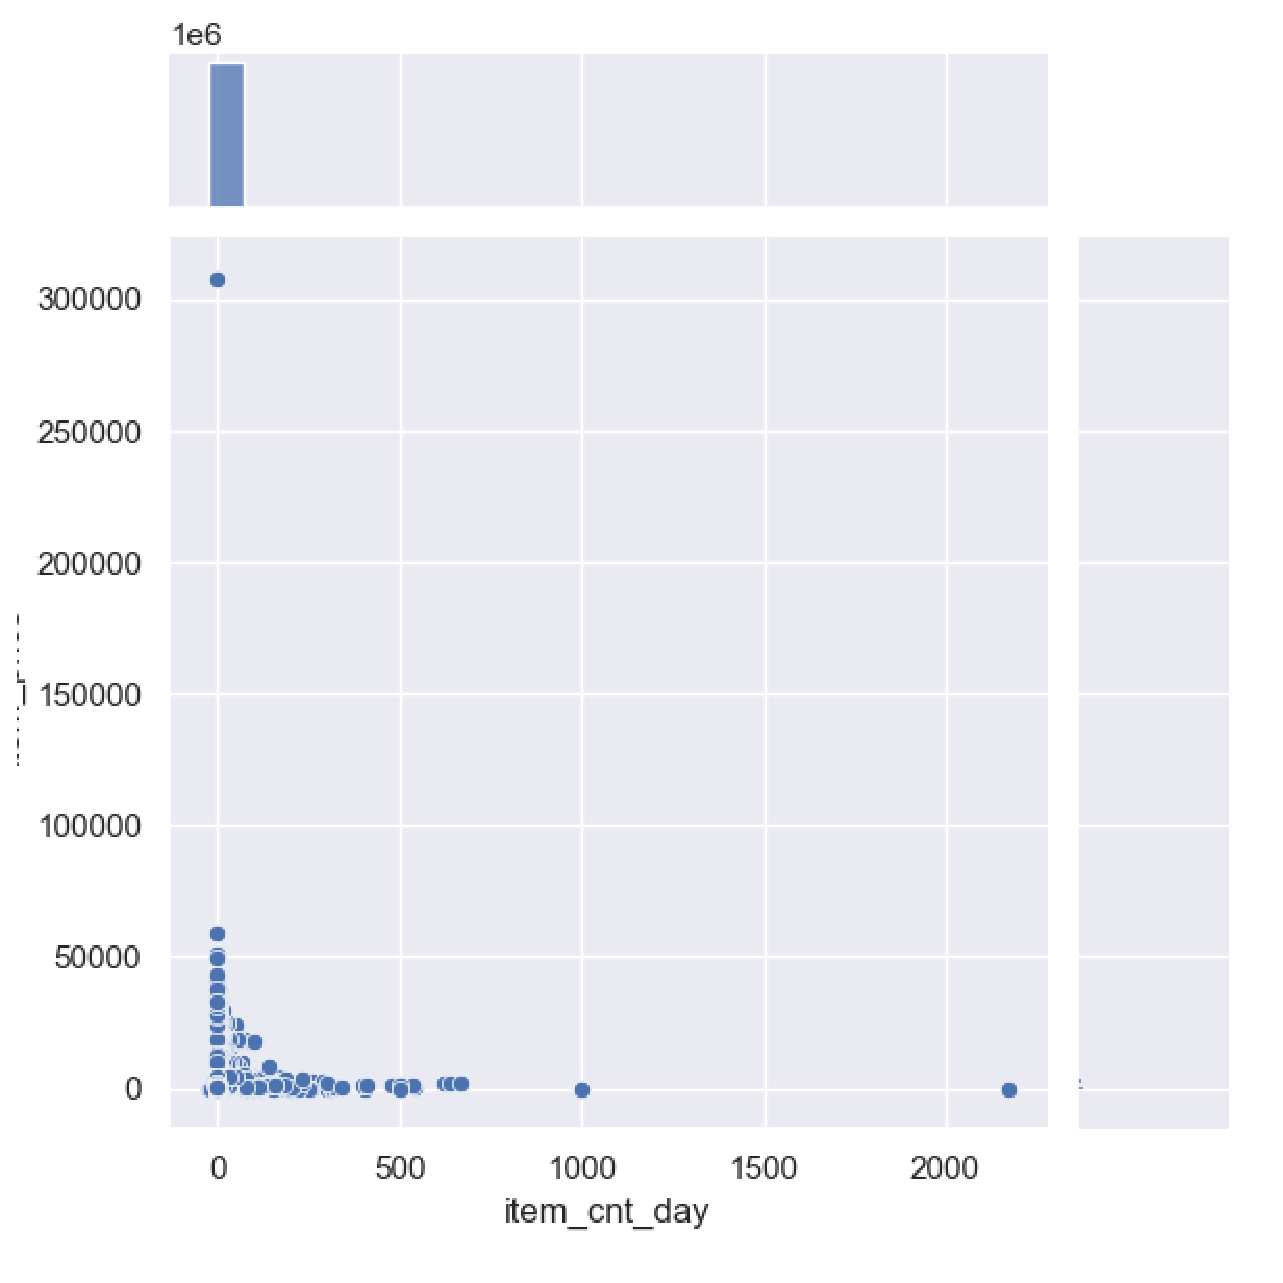
\includegraphics[width=0.8\textwidth]{logos/filter1.eps}
%     \vspace{0.4em}
%     \caption{Distribution}
%   \end{minipage}
%   \begin{minipage}[t]{0.48\textwidth}
%     \centering
%     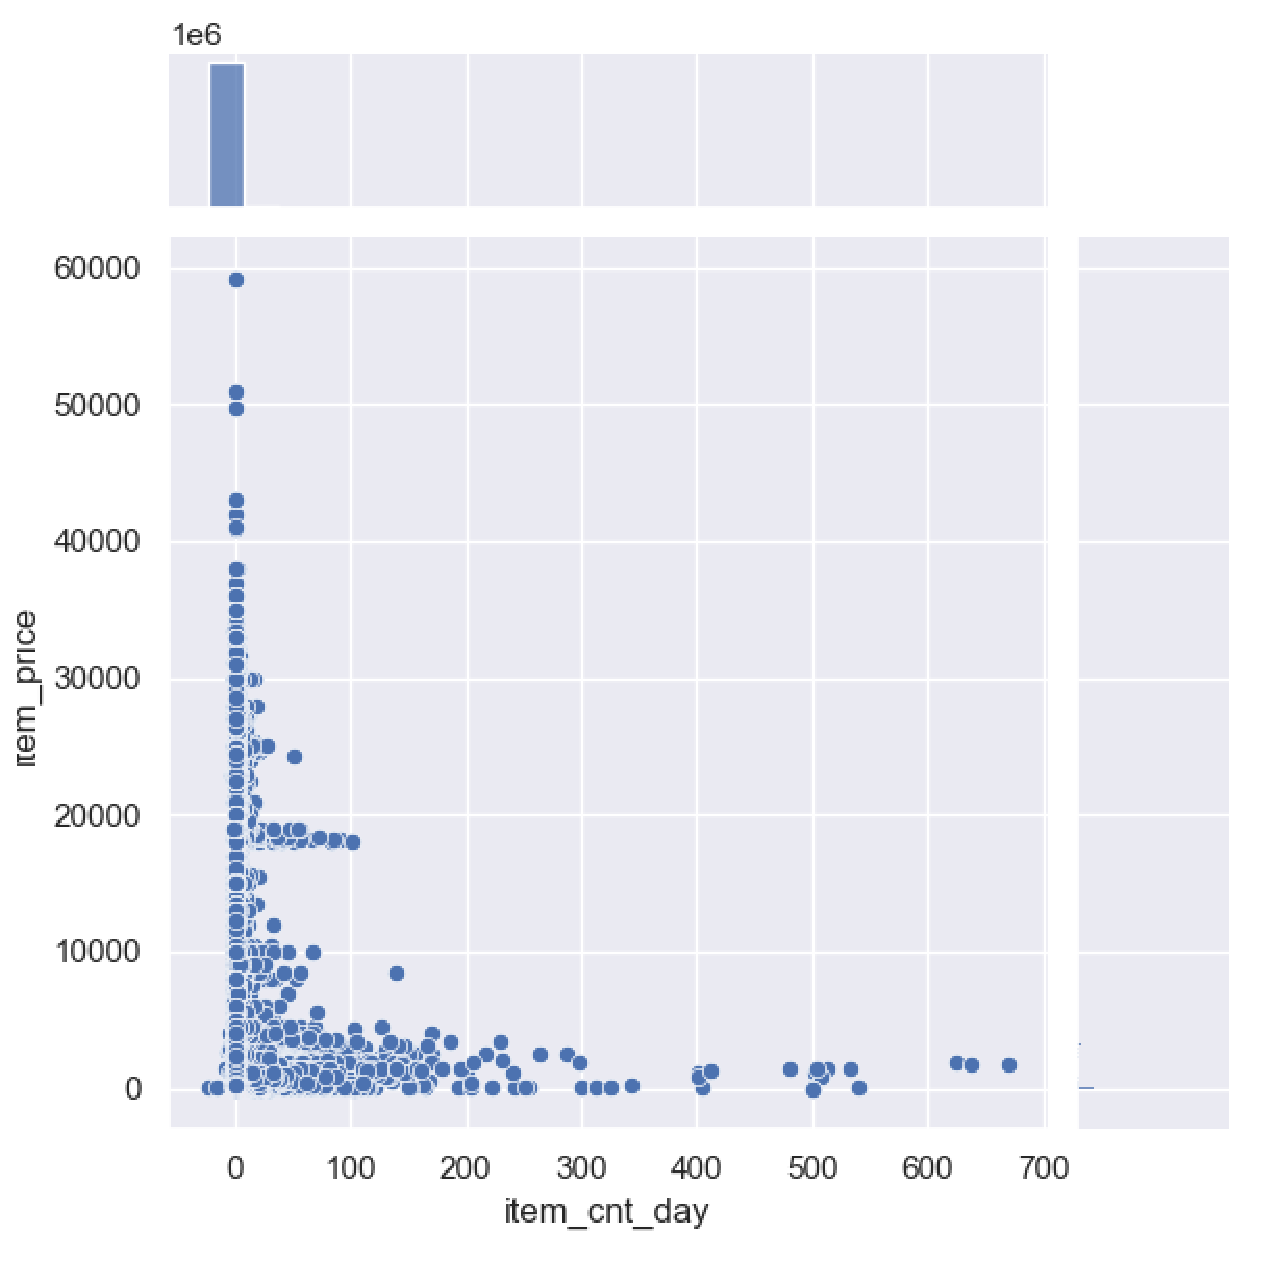
\includegraphics[width=0.8\textwidth]{logos/3.2.2.eps}
%     \vspace{0.4em}
%     \caption{Filter Abnormal}
%   \end{minipage}
% \end{figure}


%%==========================================================================================
\begin{note}
In conclusion,
we firstly formalized the problem of
group outlying aspects mining,

Then proposed a novel method GOAM algorithm to address the problem of
group outlying aspects mining,
and the proposed method use pruning to reduce time complexity
while identifying the suitable set of outlying features for the interested group.

Thank you and any question?
\end{note}
%%==========================================================================================

\end{slide}
%%
%%==========================================================================================

% \begin{slide}{Feature Analysis}
%   There are also some wrong locations in the data set. After analysis, we 
%   found a total of 67 wrong messages, which also means that we cannot use
%    these 67 wrong messages.
%   \begin{figure}
%     \centering
%     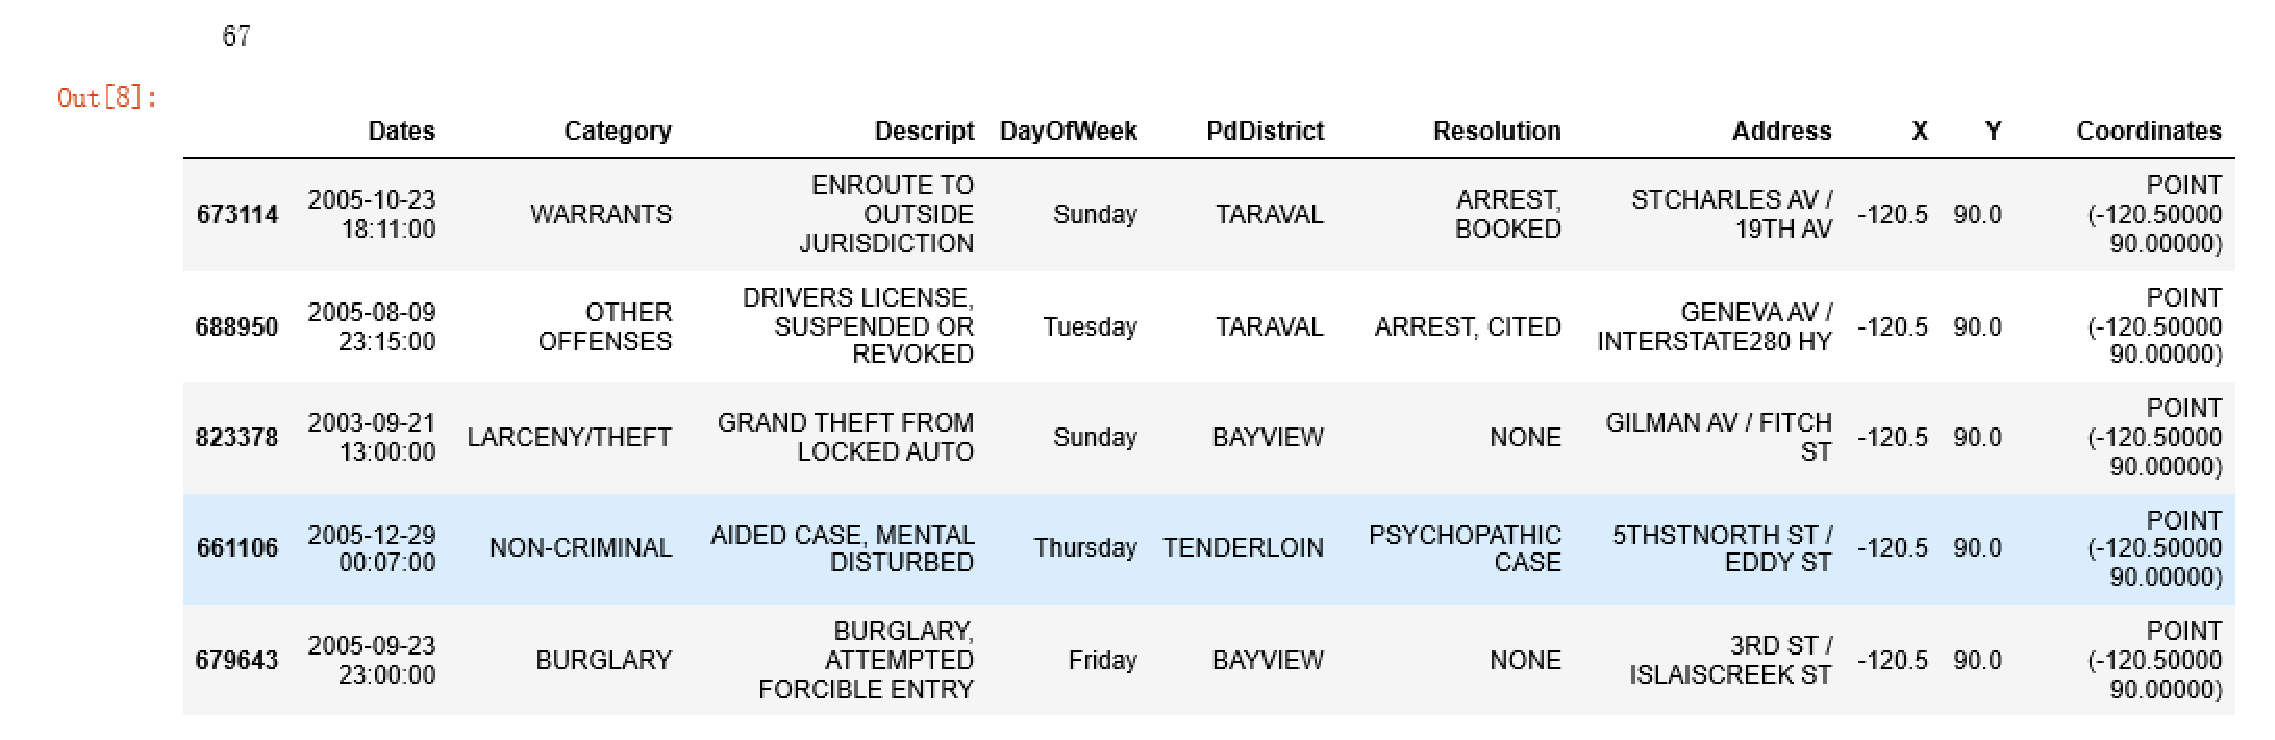
\includegraphics[width=1\textwidth]{kaggle/6.1.eps}
%   \end{figure}


% \end{slide}
%%
%%===========================================================================================
\begin{slide}{Import The Stop Lexicon}
  
  \begin{itemize}
  \item 
  You need to determine how to deal with frequent words that don't make sense.
  A stop-word database is not helpful for emotion analysis. 
  These words are called "stop-words".
  In English, they include words like "a", "and", "is" and "the".  
\end{itemize}
\begin{figure}[htbp]
  \centering
  \begin{minipage}[t]{0.58\textwidth}
    \centering
    \centerline{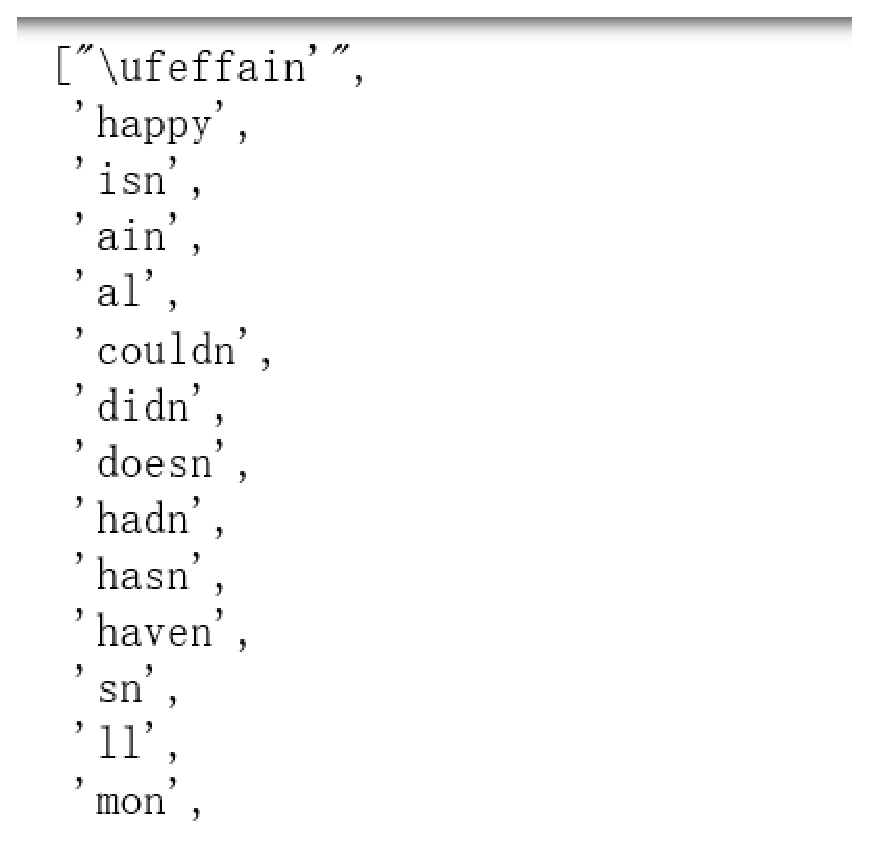
\includegraphics[width=0.68\textwidth]{logos/stop.eps}}
    \vspace{-1.0em}
    %\caption{Sales Analysis}
  \end{minipage}
\end{figure}
\end{slide}


%%
%%========================================================================

% \begin{slide}{Dates \& Day of the week}
%   These variables are distributed uniformly between 1/1/2003 to 5/13/2015 (and Monday to Sunday) and split between the training and the testing dataset as mentioned before. We did not notice any anomalies on these variables.
%   The median frequency of incidents is 389 per day with a standard deviation of 48.51.
%   Also, there is no significant deviation of incidents frequency 
%   throughout the week. Thus we do not expect this variable to play a 
%   significant role in the prediction.


%   \begin{figure}[htbp]
%     \centering
%     \begin{minipage}[t]{0.48\textwidth}
%       \centering
%       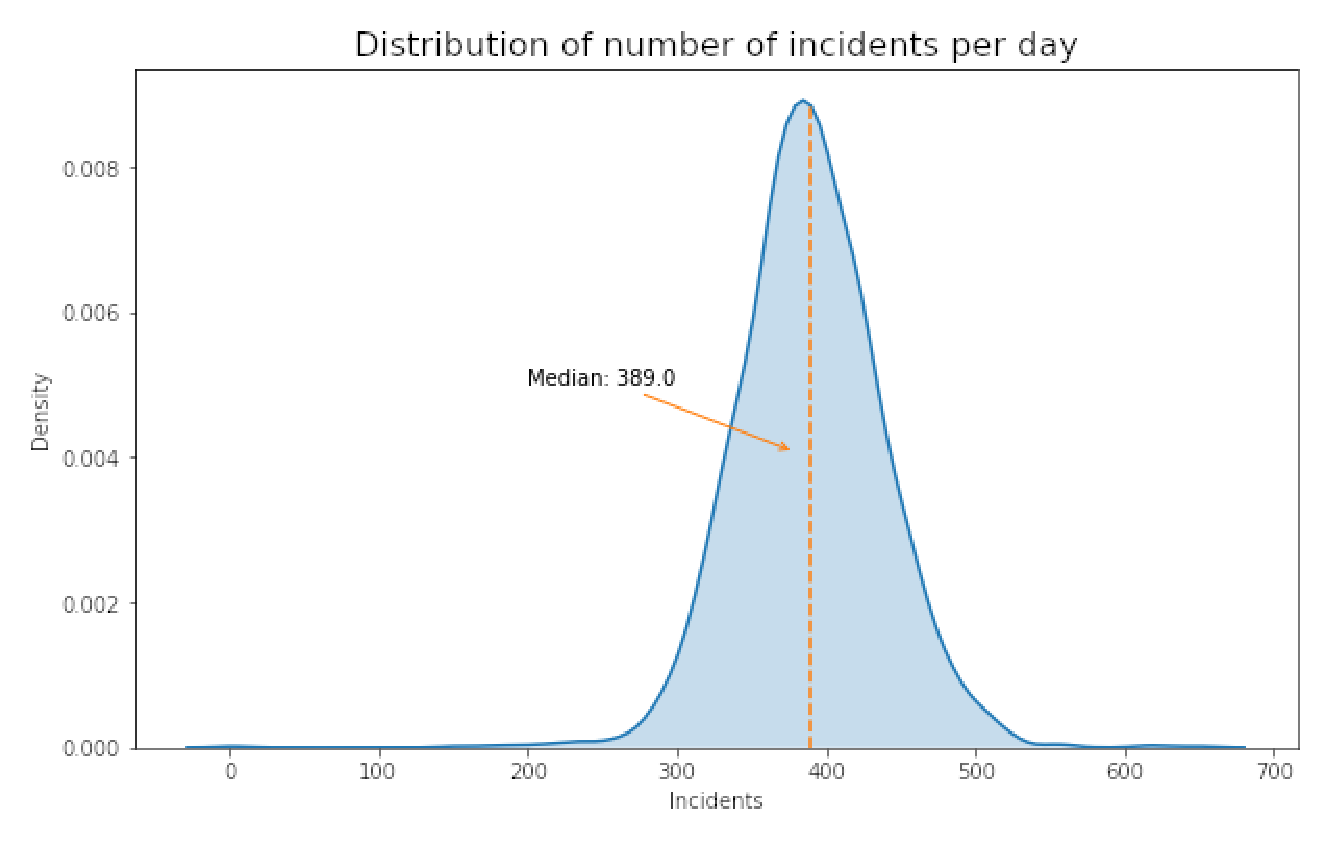
\includegraphics[width=0.8\textwidth]{kaggle/7.1.eps}
%       \vspace{0.4em}
%       \caption{Dates and Day of the Week}
%     \end{minipage}
%     \begin{minipage}[t]{0.48\textwidth}
%       \centering
%       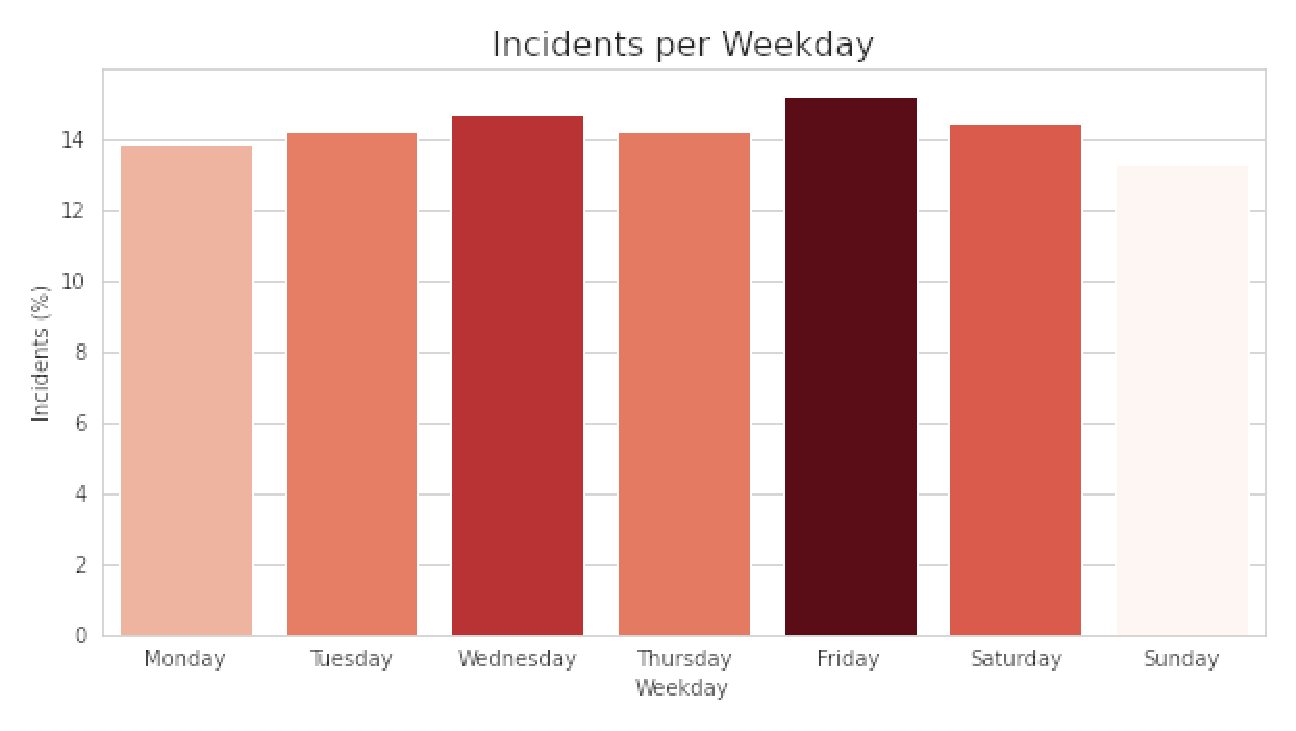
\includegraphics[width=0.8\textwidth]{kaggle/8.1.eps}
%       \vspace{0.4em}
%       \caption{Per Weekday}
%     \end{minipage}
%   \end{figure}
% \end{slide}

%%
%%%%===============================================================

%%
%%===================================================================



% \begin{slide}{Category \& Police District}
%   There are 39 discrete categories that the police department file the incidents with the most common being 
%   Larceny/Theft (19.91\%), Non/Criminal (10.50\%), and Assault(8.77\%).
%   There are significant differences between the different districts of the City with the Southern district 
%   having the most incidents (17.87\%) followed by Mission (13.67\%) and Northern (12.00\%).
%   \begin{figure}[htbp]
%     \centering
%     \begin{minipage}[t]{0.48\textwidth}
%       \centering
%       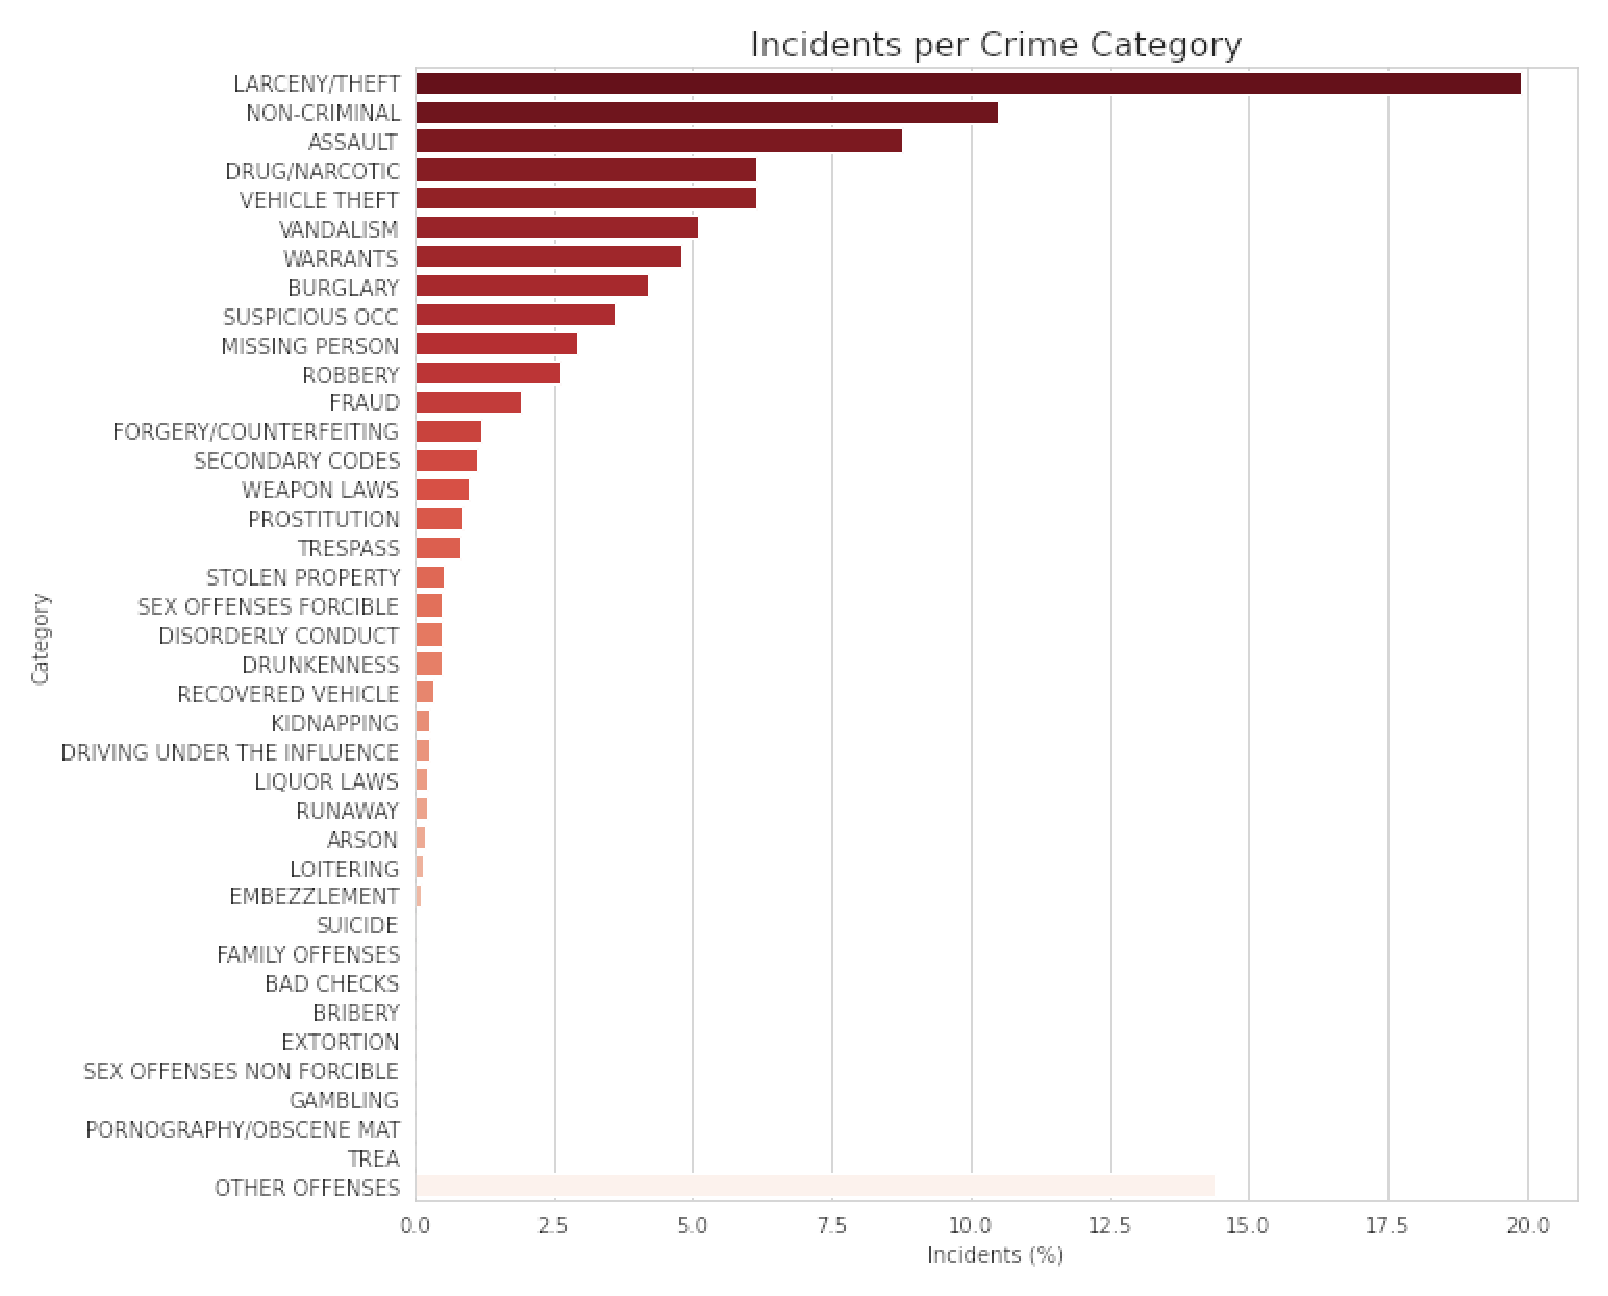
\includegraphics[width=0.7\textwidth]{kaggle/9.eps}
%       \vspace{0.4em}
%       \caption{Category}
%     \end{minipage}
%     \begin{minipage}[t]{0.48\textwidth}
%       \centering
%       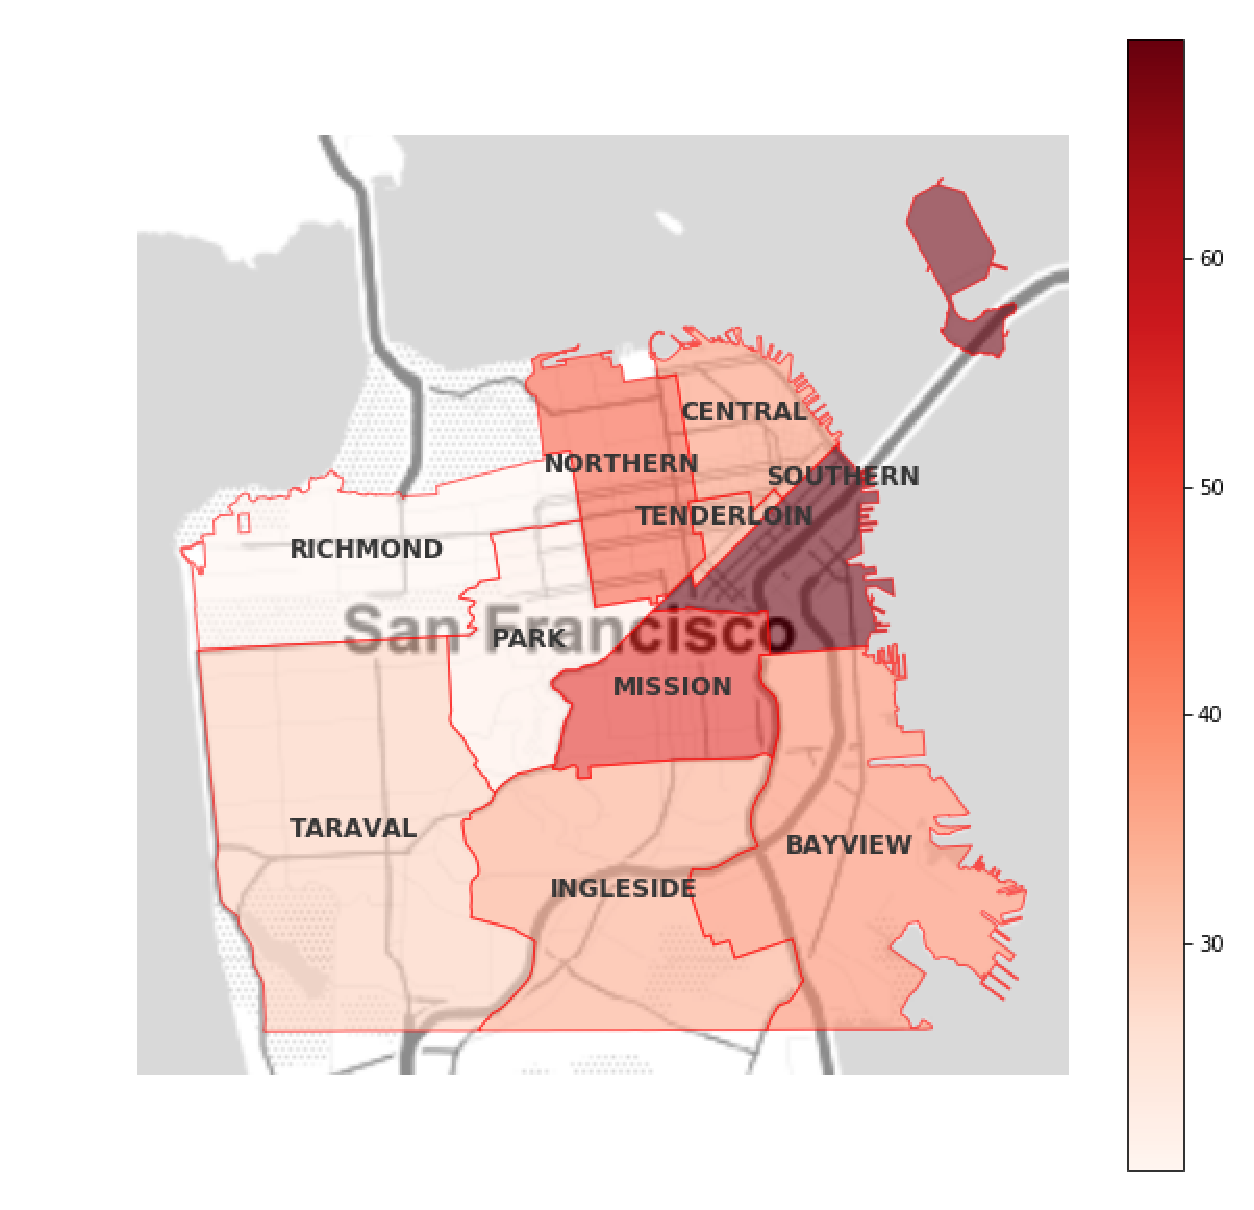
\includegraphics[width=0.7\textwidth]{kaggle/10.eps}
%       \vspace{0.4em}
%       \caption{Police District}
%     \end{minipage}
%   \end{figure}
% \end{slide}

%%
%%=========================================================================

%%
%%==========================================================================


% \begin{slide}{}
%   \begin{itemize}
%   \item Address
% Address, as a text field, requires advanced techniques to use 
% it for the prediction. Instead in this project, we will use it to 
% extract if the incident has happened on the road or in a building block.
% \item X - Longitude Y - Latitude
% We have tested that the coordinates belong inside the
%  boundaries of the city. Although longitude does not contain any
%   outliers, latitude includes some 90o values which correspond to the North Pole.
% \end{itemize}
% \end{slide}

%%
%%==============================================================================

\section{Characteristics Of The Engineering} 

%%===========================================================================================
%%

%%
%%========================================================================================

\begin{slide}{Build The Model}
  Throw these words directly to the computer, the computer can't calculate them, 
  so we need to convert the text into vectors and use the word bag model for text feature engineering.
  \\There are several common text vector processing methods, such as: word bag model,TF-IDF model,
  WORD2VEC model for text feature engineering.
  % \begin{itemize}
%   \item  Sales analysis\\
%   Overall sales were down, and monthly sales were mostly down year on year.
% One item sold exceptionally well.
%   % \item From the ‘Dates’ field, we extracted the Day, the Month, the
%   %  Year, the Hour, the Minute, the Weekday, and the number of days 
%   %  since the first day in the data.

%   % \item From the ‘Address’ field we extracted if the incident has taken
%   %  place in a crossroad or on a building block.
% \end{itemize}
% \begin{figure}[htbp]
%   \centering
%   \begin{minipage}[t]{0.28\textwidth}
%     \centering
%     \centerline{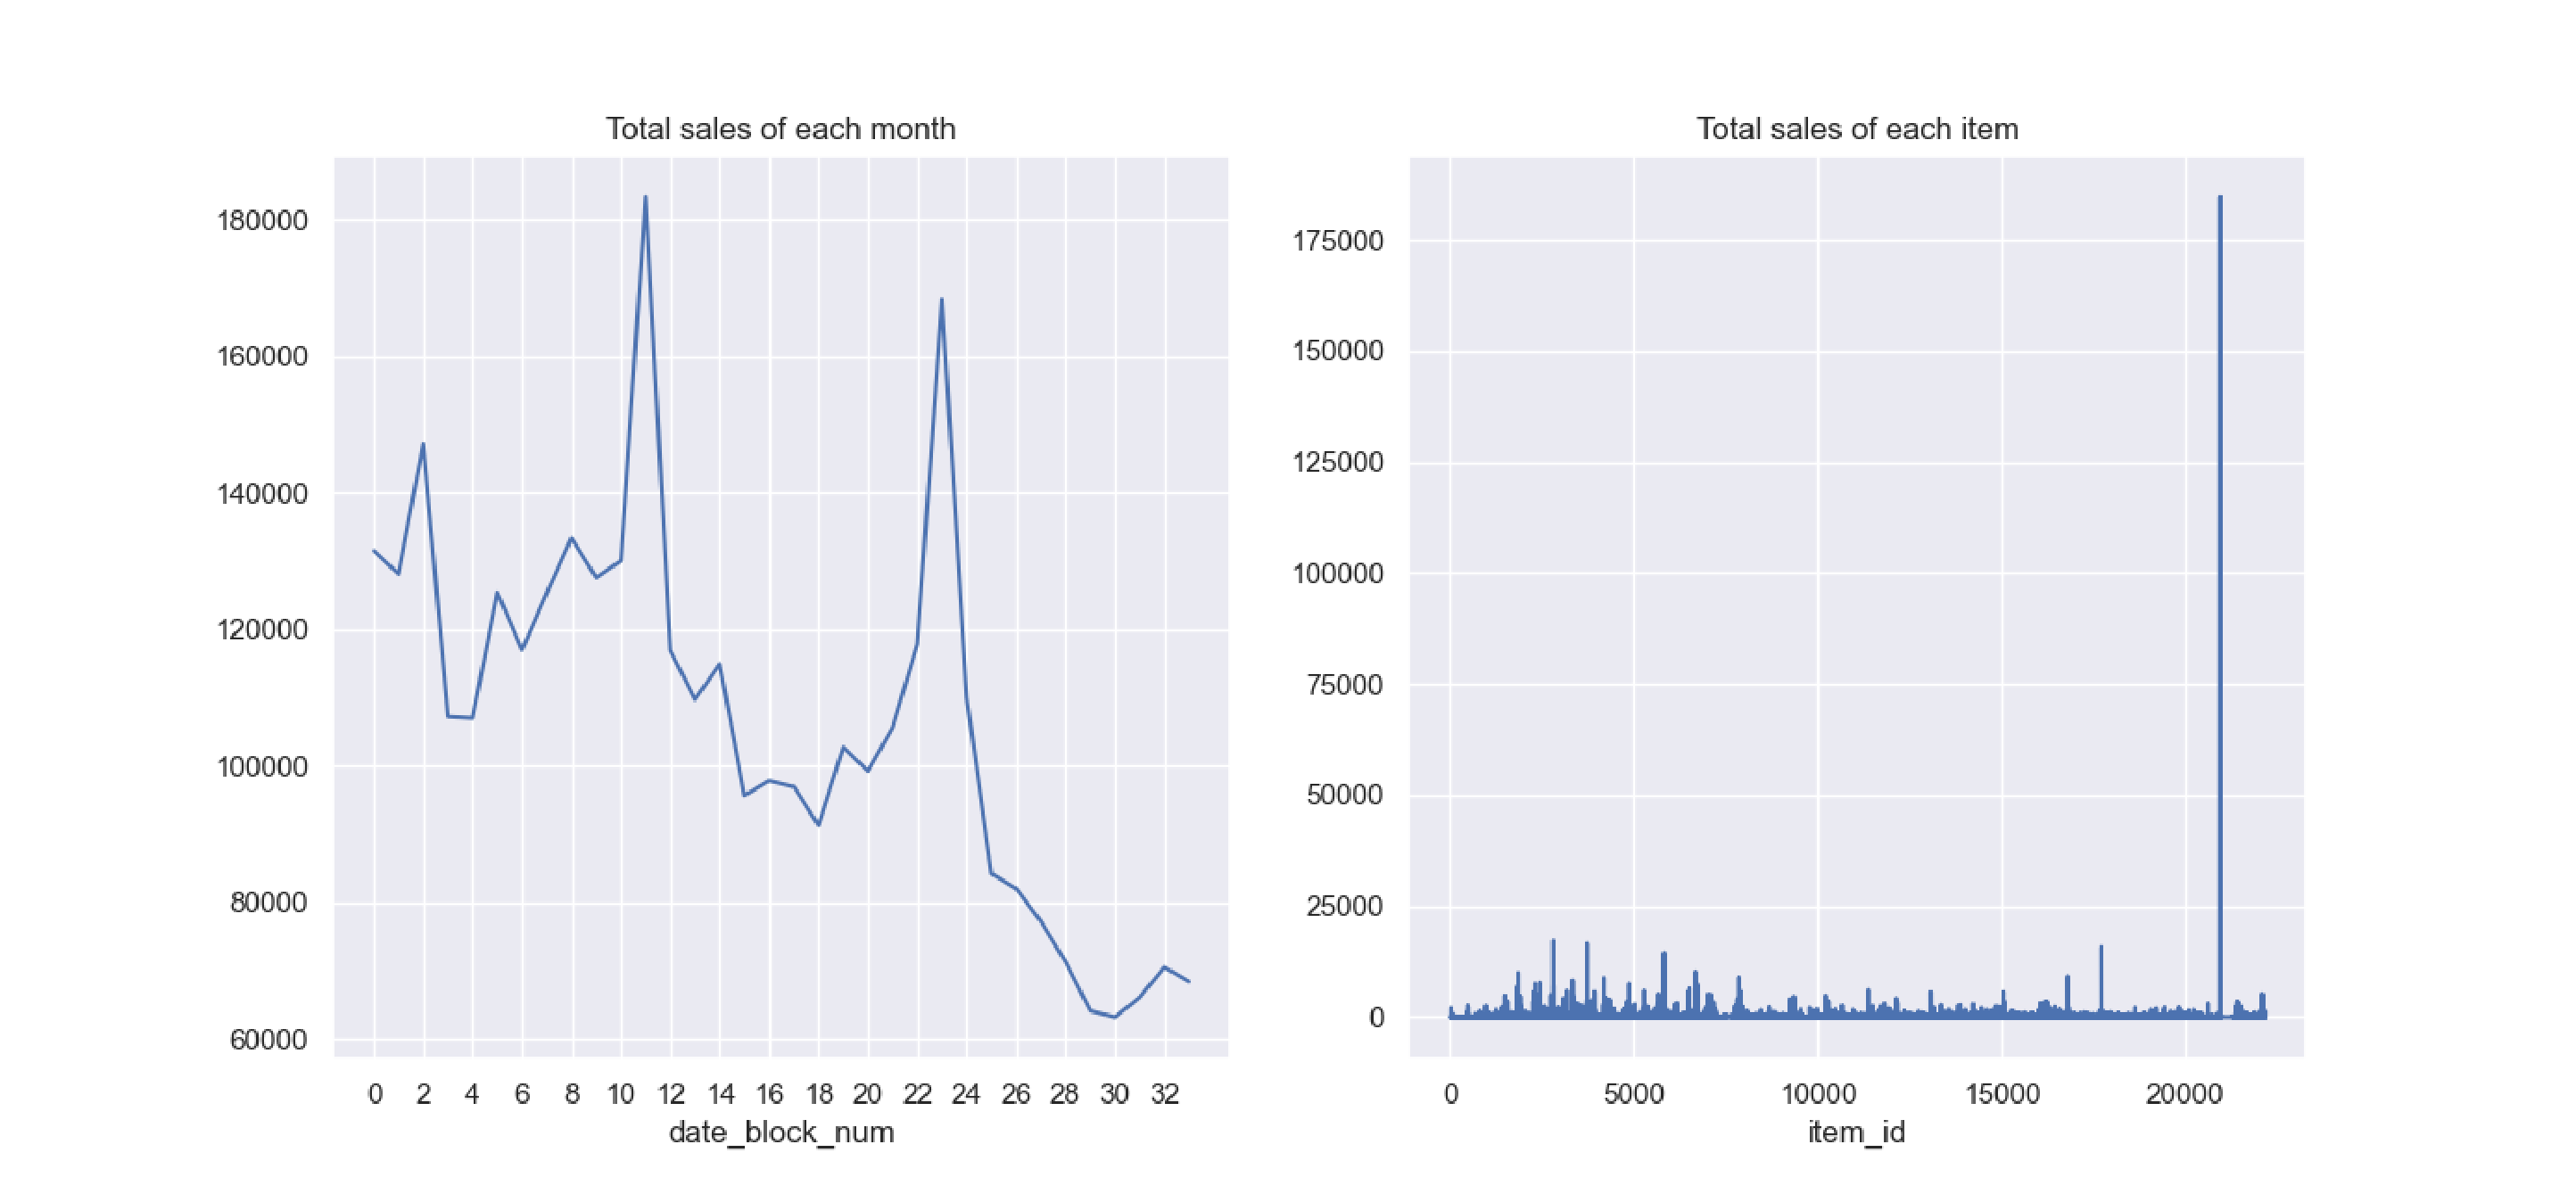
\includegraphics[width=3\textwidth]{logos/sale.eps}}
%     \vspace{-1.0em}
%     %\caption{Sales Analysis}
%   \end{minipage}
% \begin{figure}
%   \centering
%   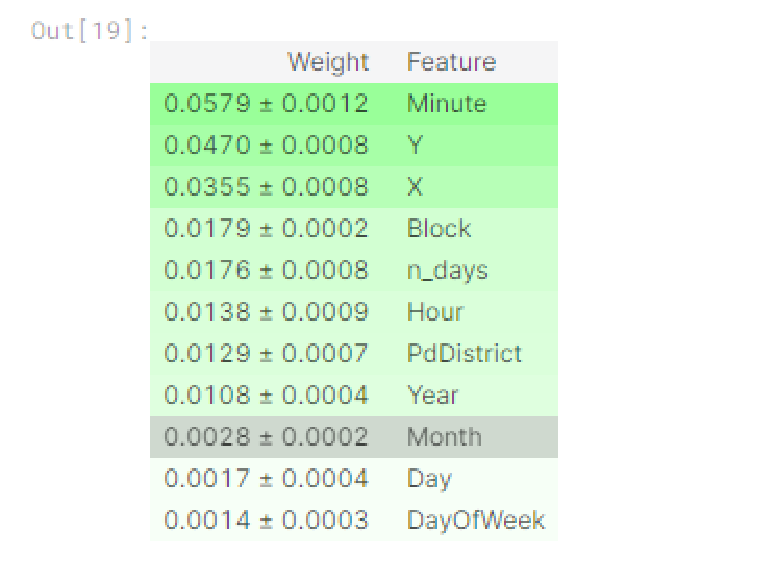
\includegraphics[width=0.5\textwidth]{kaggle/14.eps}
% \end{figure}

\end{slide}

\begin{slide}{Bag-of-words Model}
  
  \begin{itemize}
  \item  
    The word bag model learns vocabulary from all documents and then models each document
    by counting the number of occurrences of each word.
    \\The corpus is used to construct the word bag model, 
    \\and the constructed word bag model is used to carry out feature engineering 
    \\for each word in the training set and the verification set and turn it into a vector
  \end{itemize}
% \begin{figure}[htbp]
%   \centering
%   \begin{minipage}[t]{0.28\textwidth}
%     \centering
%     \centerline{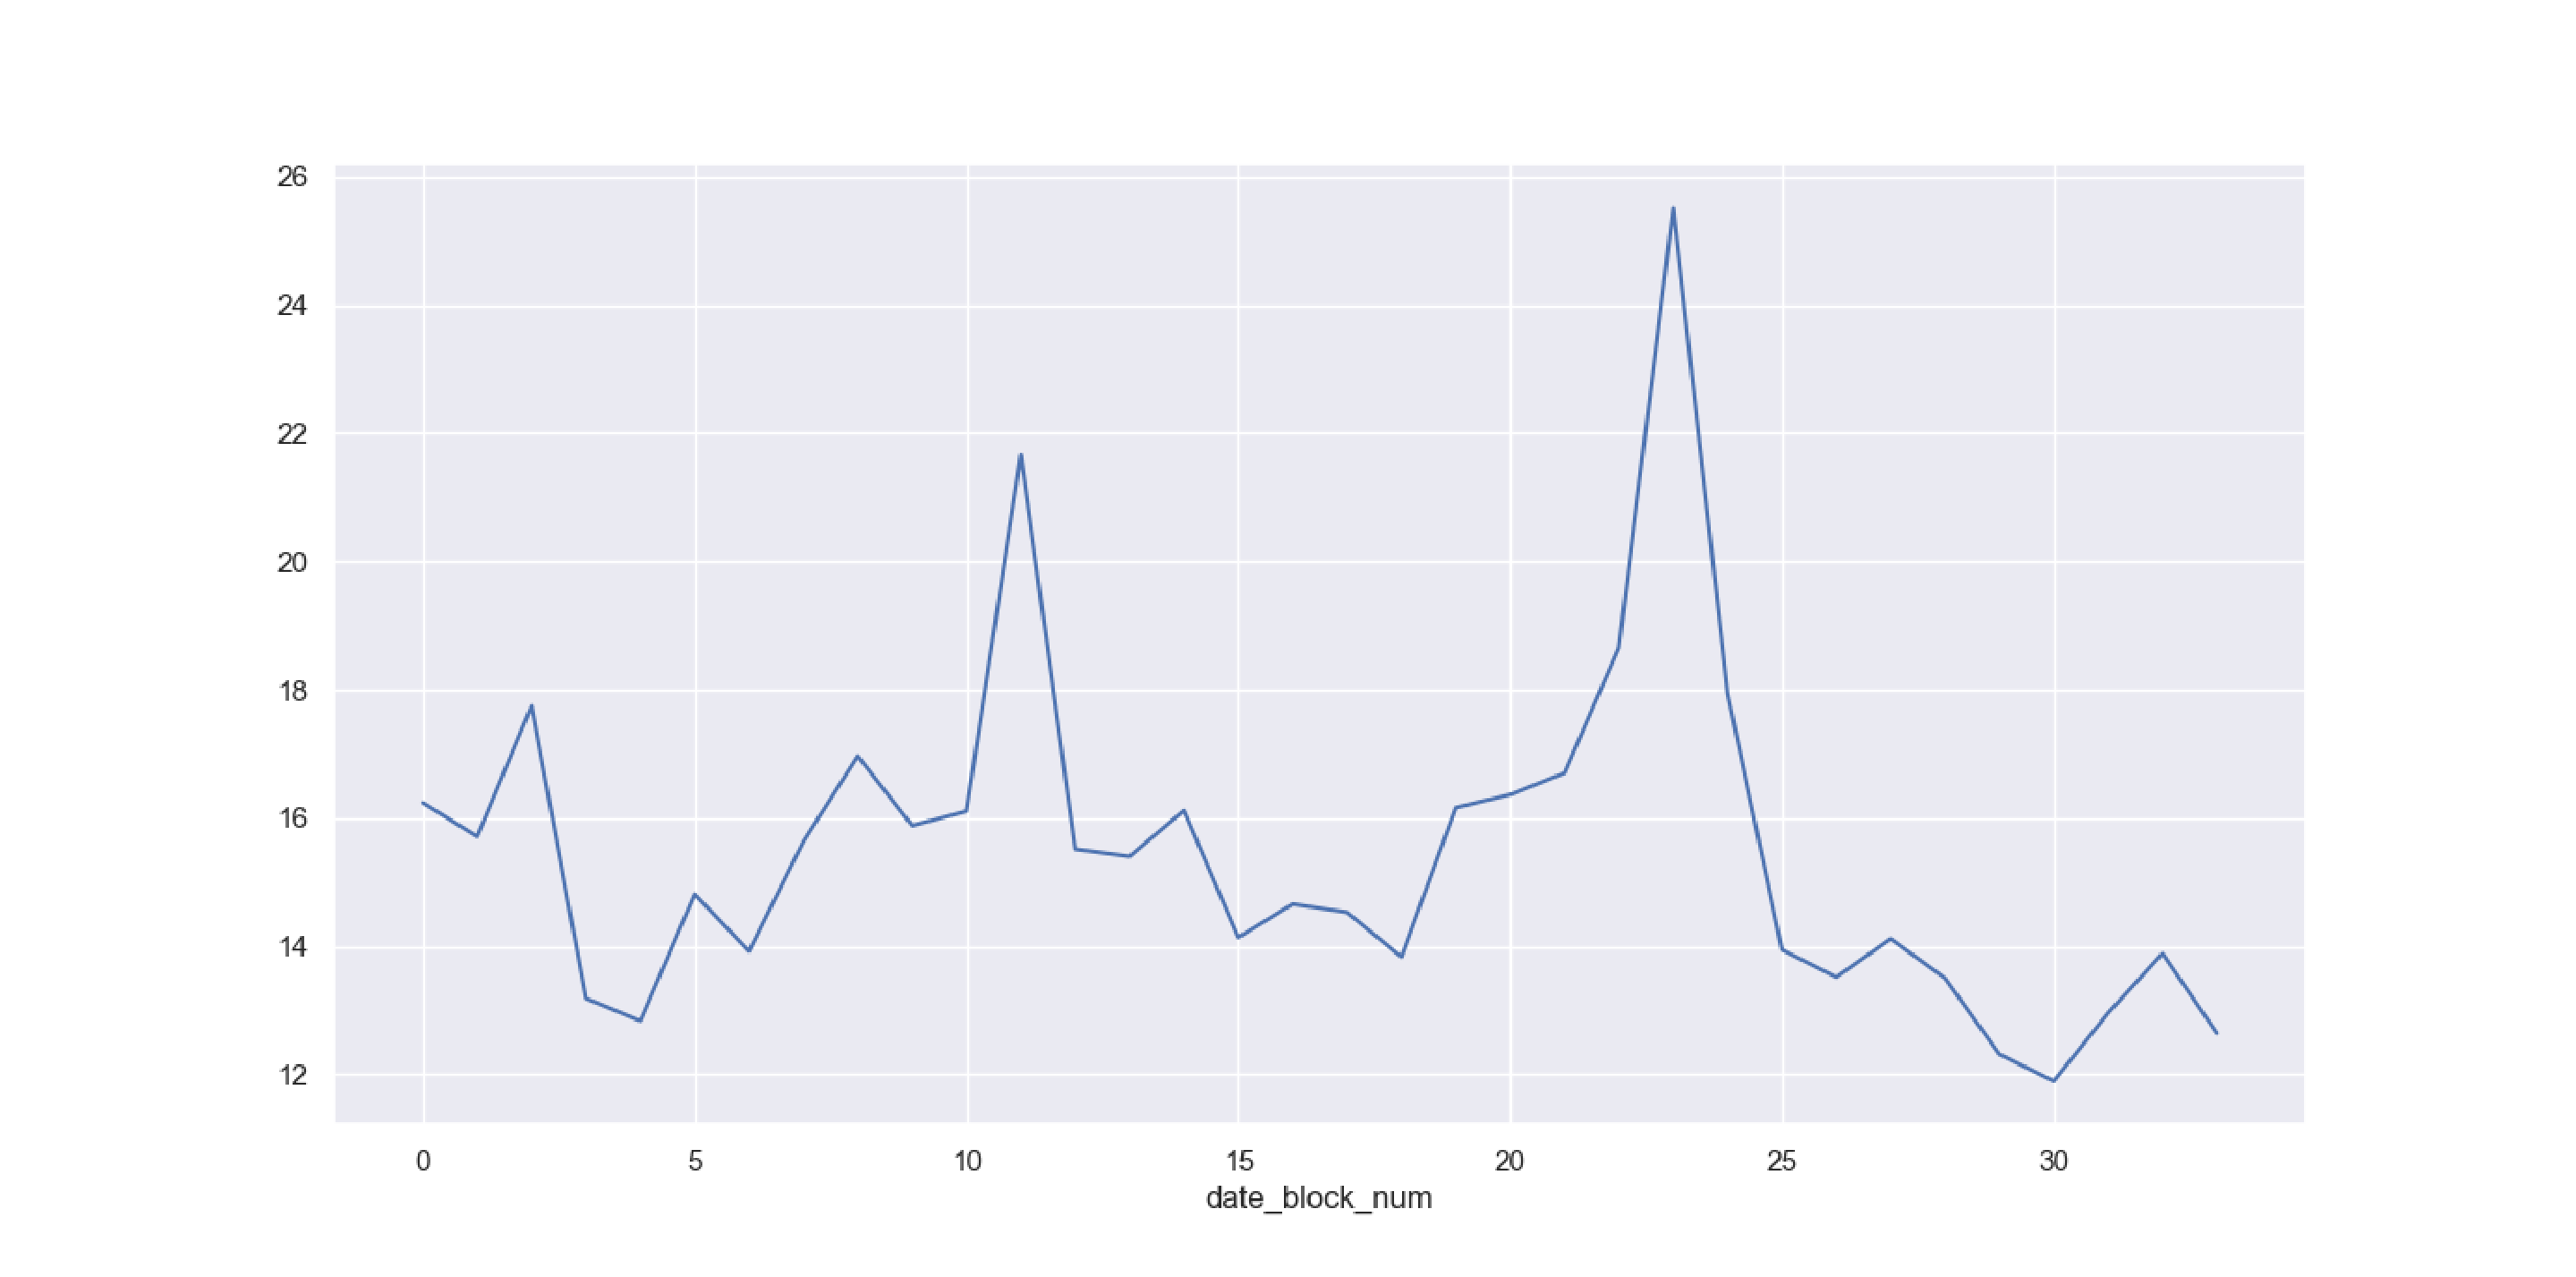
\includegraphics[width=3\textwidth]{logos/aveitem.eps}}
%     \vspace{-1.0em}
%     %\caption{Sales Analysis}
%   \end{minipage}
% \end{figure}
\end{slide}
%%
%%==================================================================================
\begin{slide}{TF-IDF Model}
  
  \begin{itemize}
  \item  
    TF-IDF is a statistical method used to assess the importance of a word to one of the documents 
    in a document set or corpus.
    \\The importance of a word increases proportionally with the frequency of its occurrence in the document, 
    but decreases inversely with the frequency of its occurrence in the corpus.
    \\Word frequency (TF) represents the frequency of entries (keywords) in the text.
  \end{itemize}
% \begin{figure}[htbp]
%   \centering
%   \begin{minipage}[t]{0.28\textwidth}
%     \centering
%     \centerline{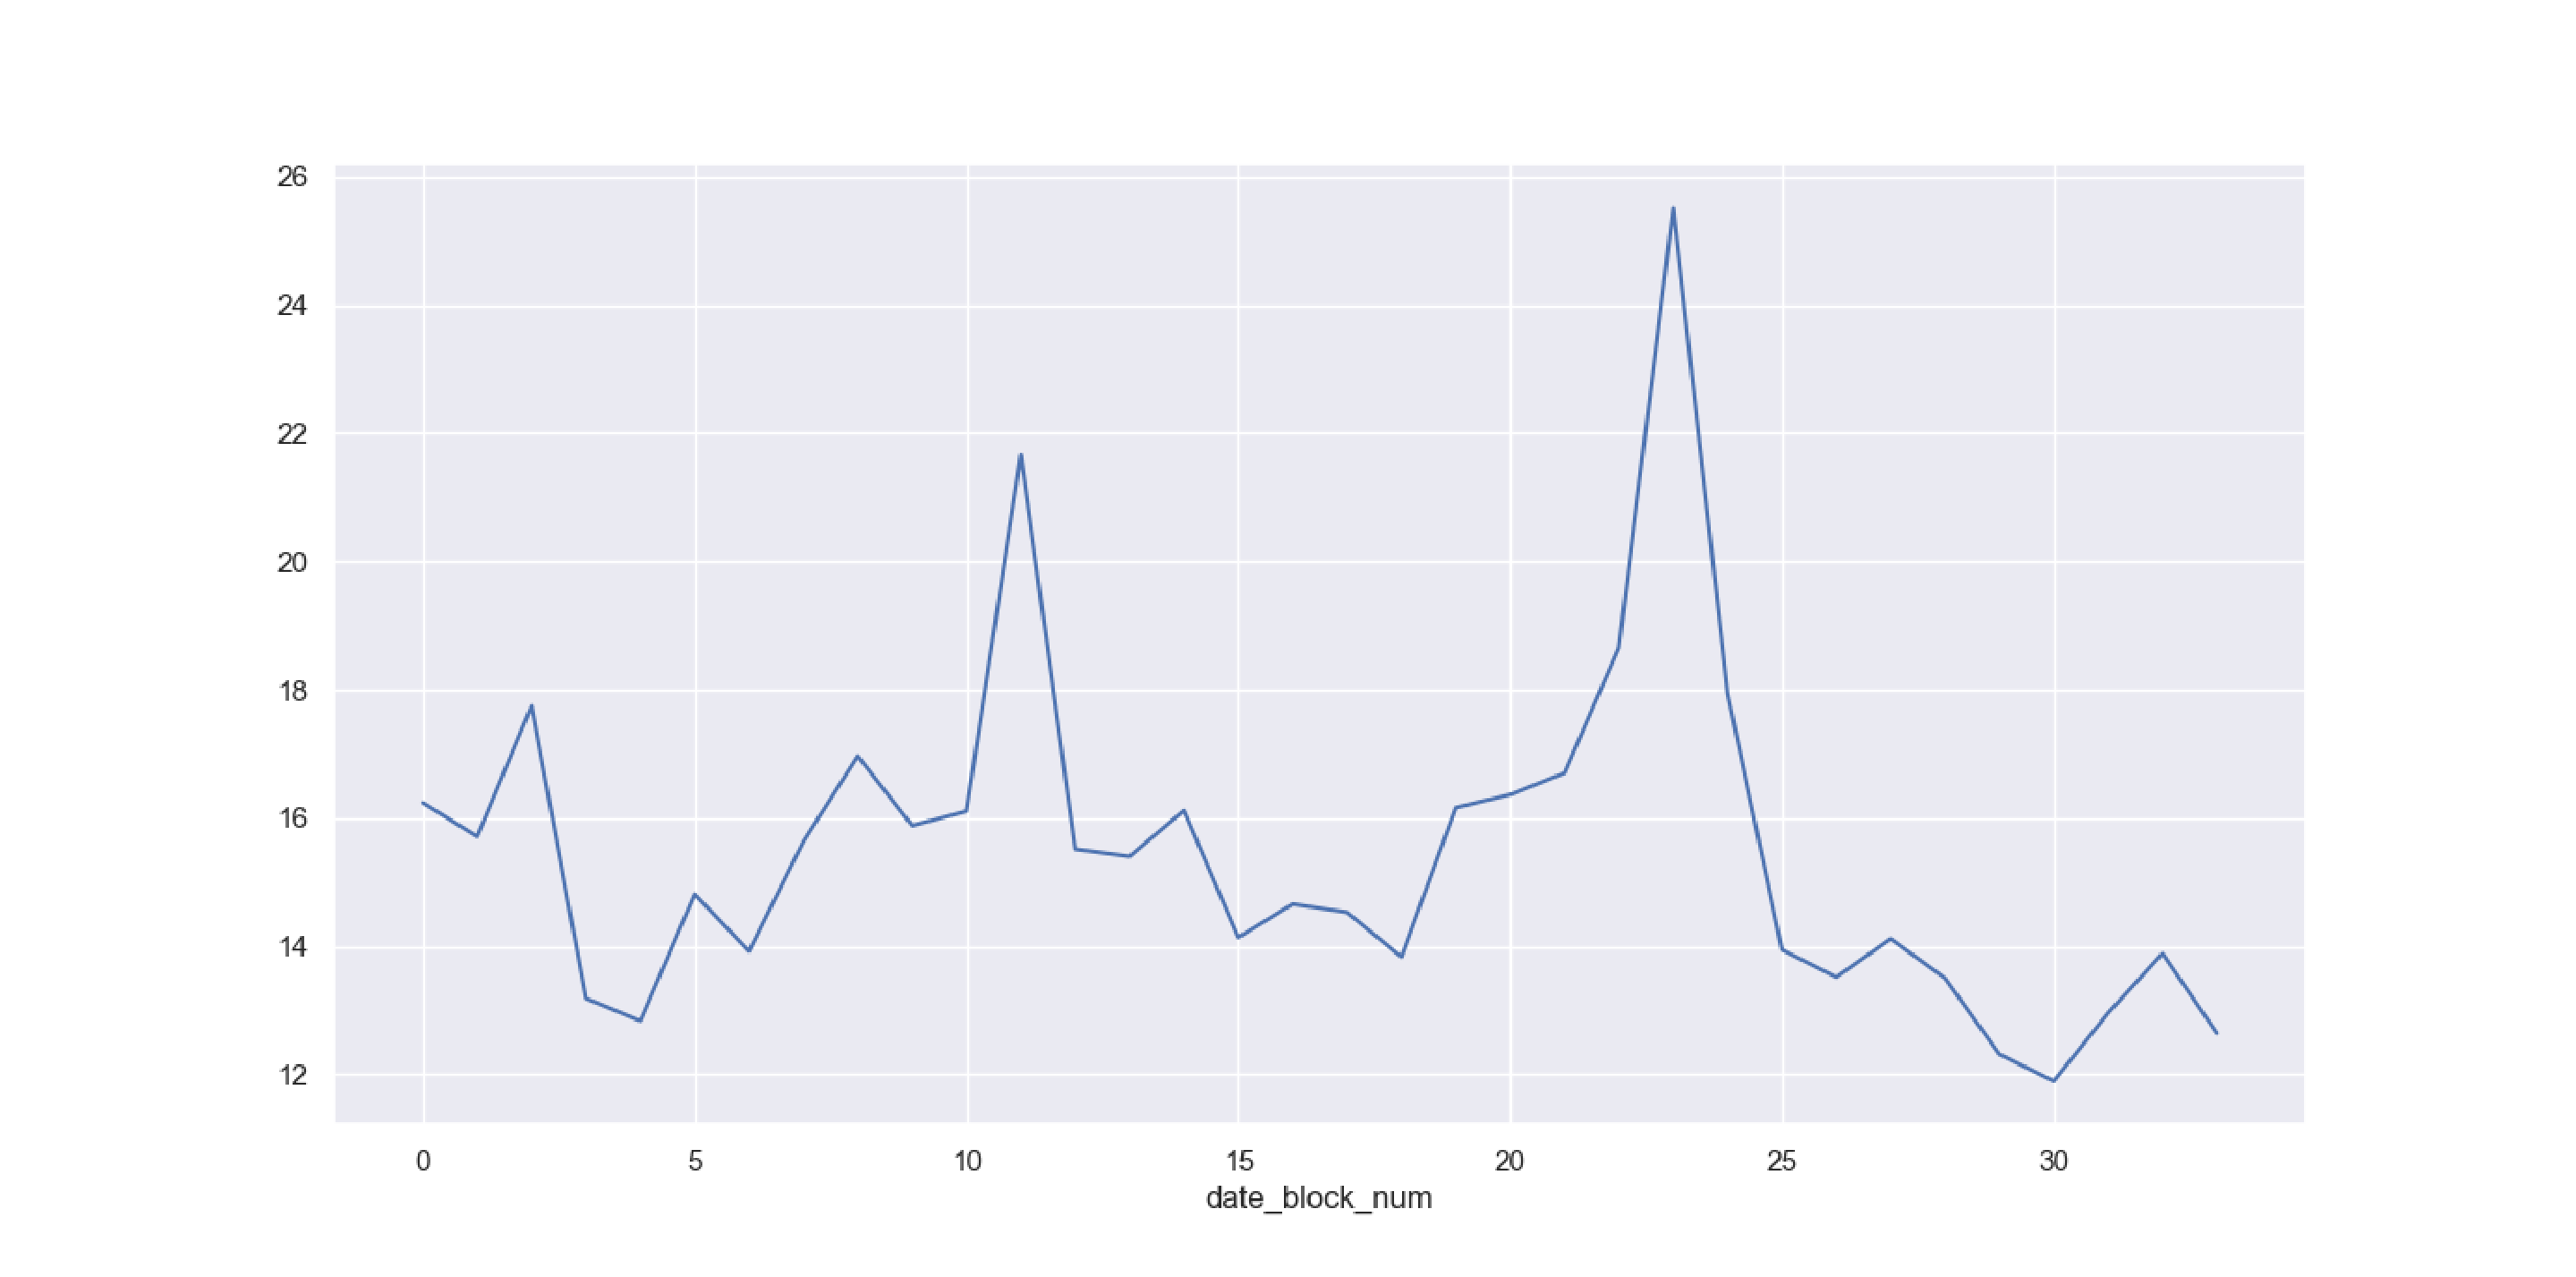
\includegraphics[width=3\textwidth]{logos/aveitem.eps}}
%     \vspace{-1.0em}
%     %\caption{Sales Analysis}
%   \end{minipage}
% \end{figure}
\end{slide}

\section{Construct The Classifier Algorithm}

%%
%%============================================================================================

%%
%%==============================================================================================
\begin{slide}{Classifier Algorithm}
  \begin{itemize}
    \item  
    Machine learning and data mining are carried out for the text processed by the word bag model.
    \\Use the logistic regression activation function to convert the output label of the category variable to a numeric variable.
   \\ The word bag method was used for text feature engineering, and sklearn default logistic regression classifier was used to verify the prediction accuracy on the set.
  %\item  Display of test data
  \end{itemize}
  
  % \begin{figure}[htbp]
  %   \centering
  %   \begin{minipage}[t]{0.28\textwidth}
  %     \centering
  %     \centerline{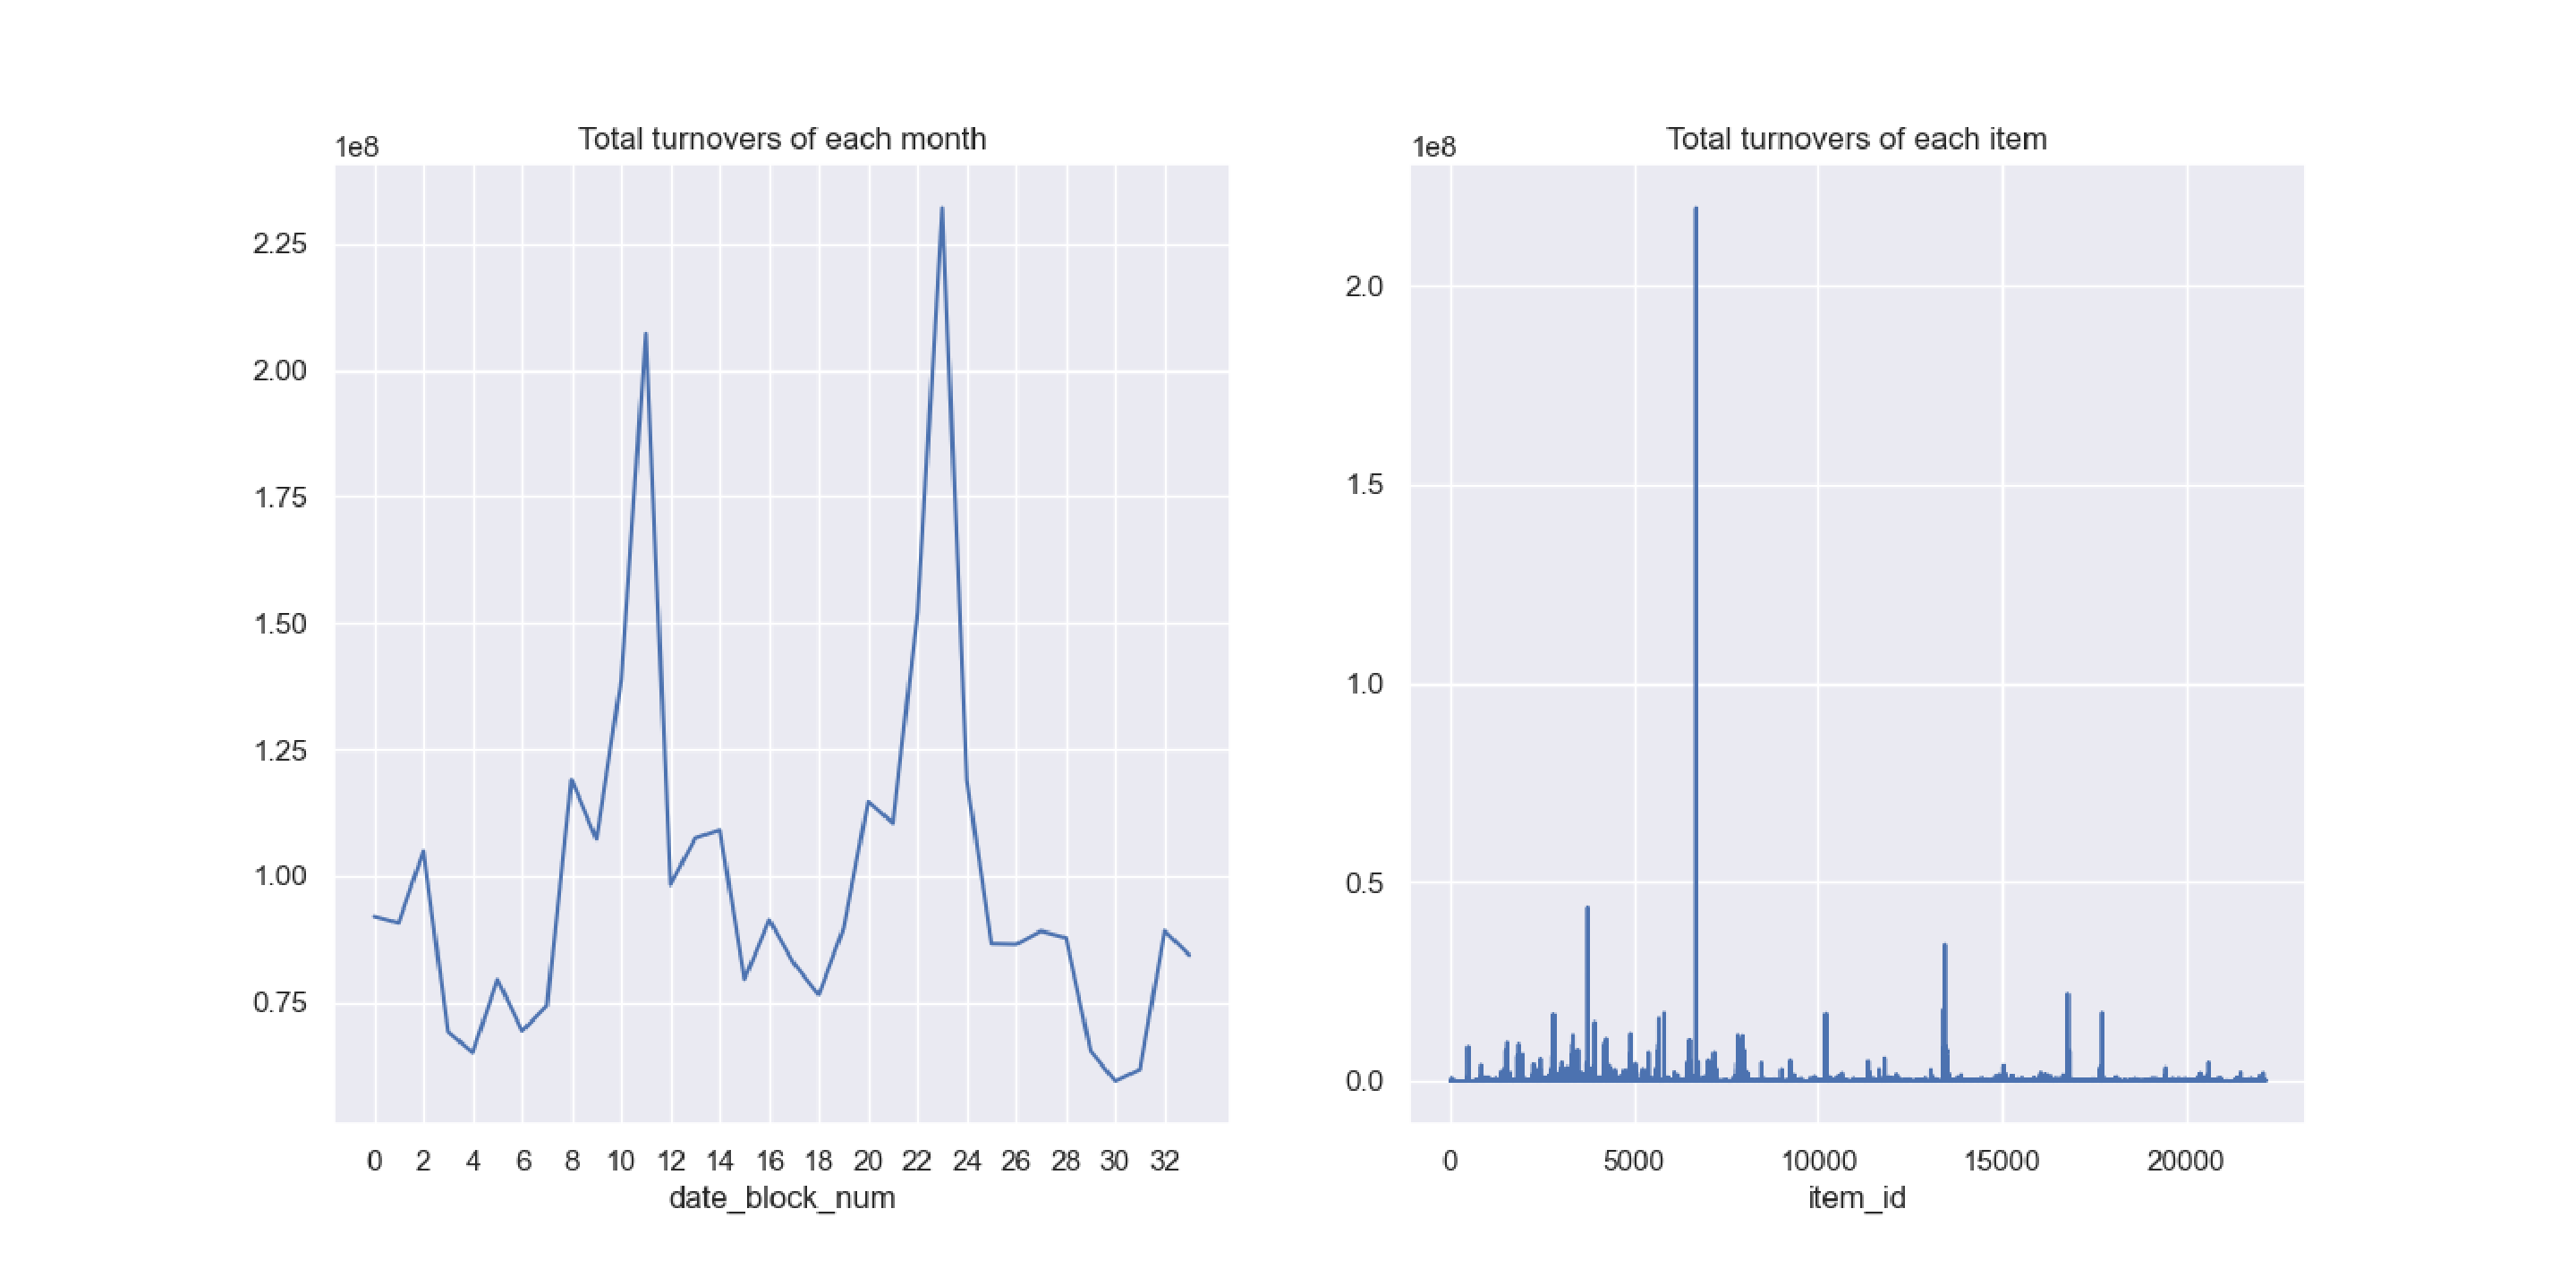
\includegraphics[width=3\textwidth]{logos/turnover.eps}}
  %     \vspace{-1.0em}
  %     %\caption{precdtion}
  %   \end{minipage}
  % \end{figure}
\end{slide}

% \begin{slide}{Profit  Analysis}
%   \begin{itemize}
%     \item The highest-grossing commodity\\
%     The number one item in total revenue accounts for a percentage of monthly revenue
%   %\item  Display of test data
%   \end{itemize}
  
%   \begin{figure}[htbp]
%     \centering
%     \begin{minipage}[t]{0.28\textwidth}
%       \centering
%       \centerline{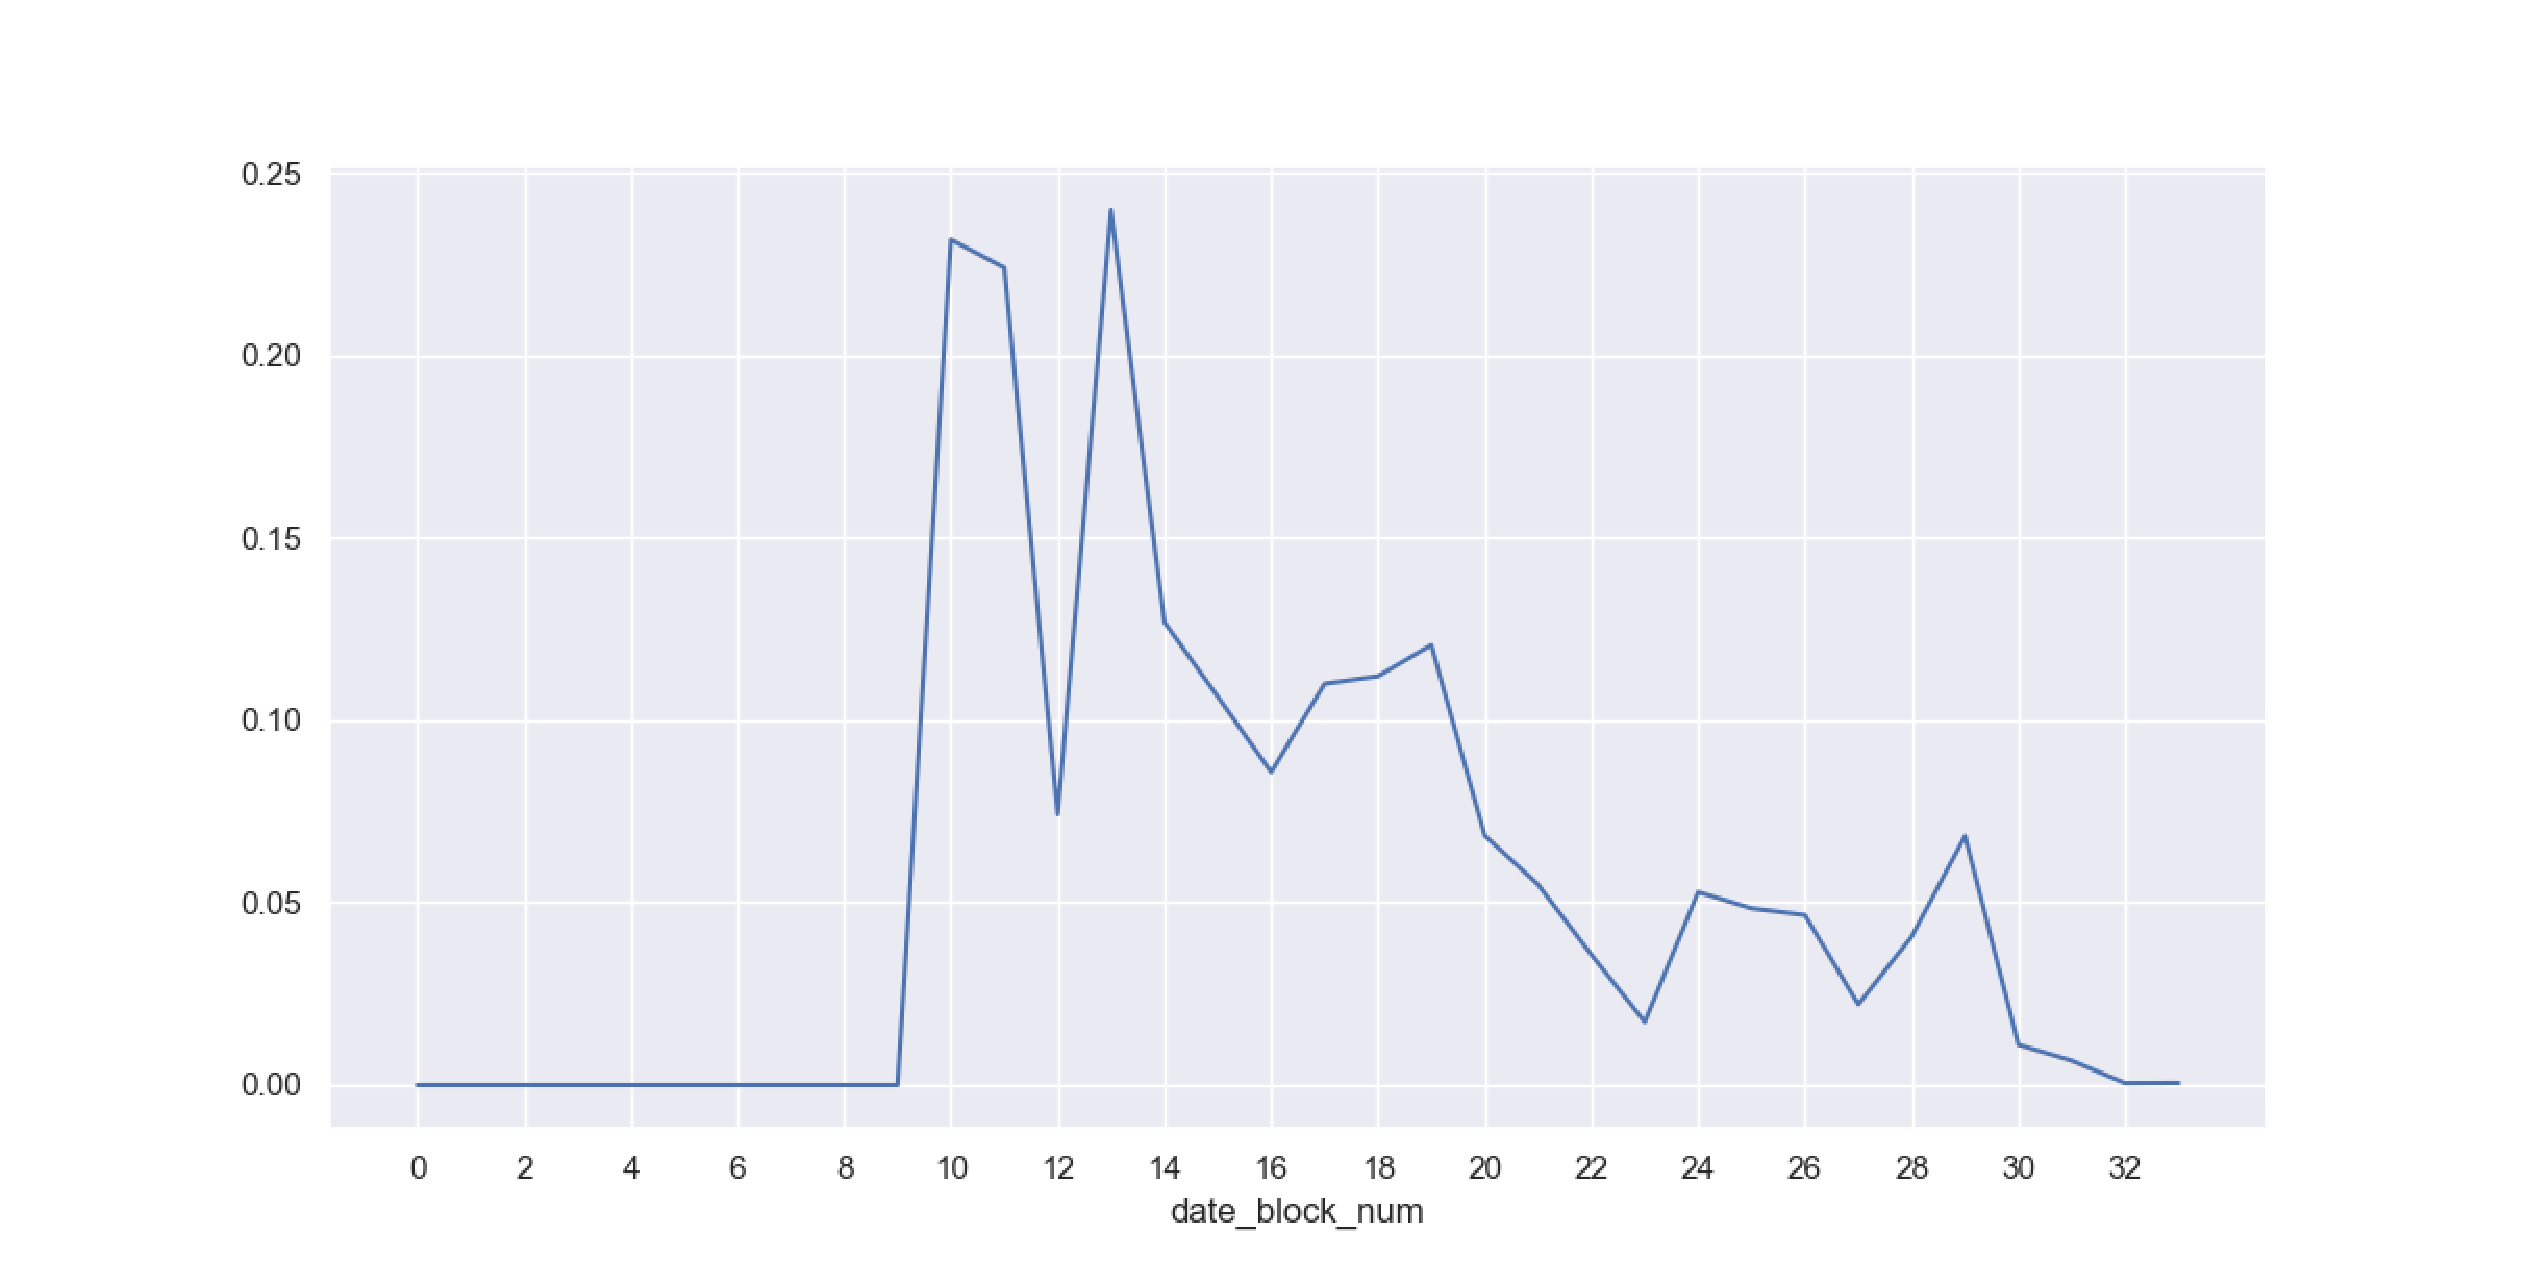
\includegraphics[width=3\textwidth]{logos/highcom.eps}}
%       \vspace{-1.0em}
%       %\caption{precdtion}
%     \end{minipage}
%   \end{figure}
% \end{slide}

%%
%%==============================================================================
\section{Predict Test Set Data}
\begin{slide}{Predict Test Set Data}
\begin{itemize}
 \item 
  The text in the test set was predicted using the LG_FINAL logistic regression classifier, 
\\the predicted results were viewed, the test results were added to the test set, 
 each film comment in the test set was tagged, and submitted in the phrase ID-emotion tag format.
  % \item From the ‘Dates’ field, we extracted the Day, the Month, the
  %  Year, the Hour, the Minute, the Weekday, and the number of days 
  %  since the first day in the data.

  % \item From the ‘Address’ field we extracted if the incident has taken
  %  place in a crossroad or on a building block.
\end{itemize}
% \begin{figure}[htbp]
%   \centering
%   \begin{minipage}[t]{0.48\textwidth}
%     \centering
%     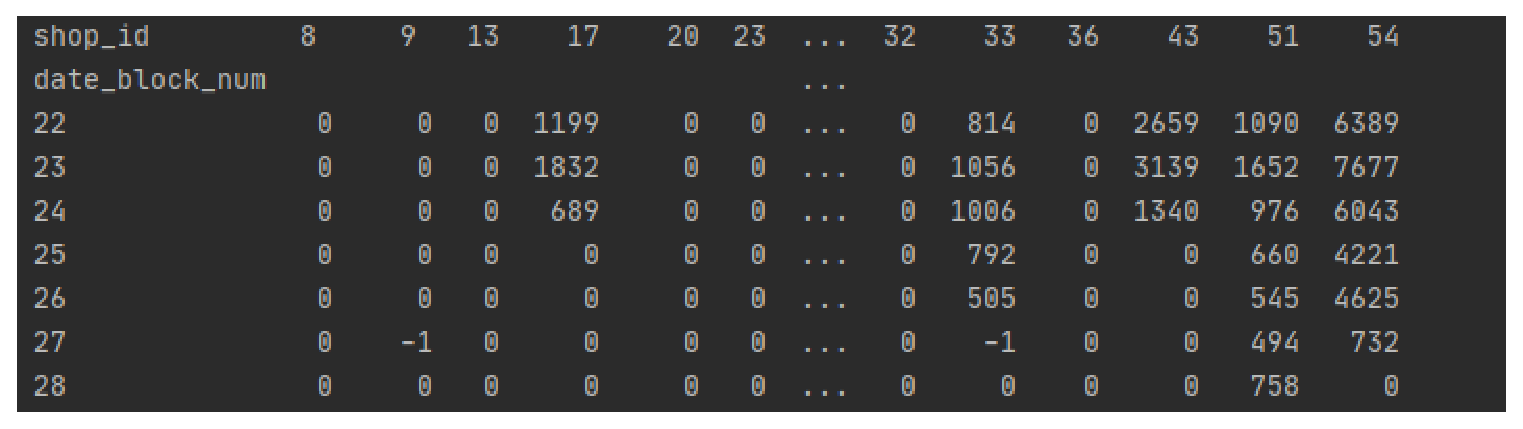
\includegraphics[width=0.88\textwidth]{logos/close.eps}
%     \vspace{0.4em}
%     \caption{Closed Stores}
%   \end{minipage}
%   \begin{minipage}[t]{0.48\textwidth}
%     \centering
%     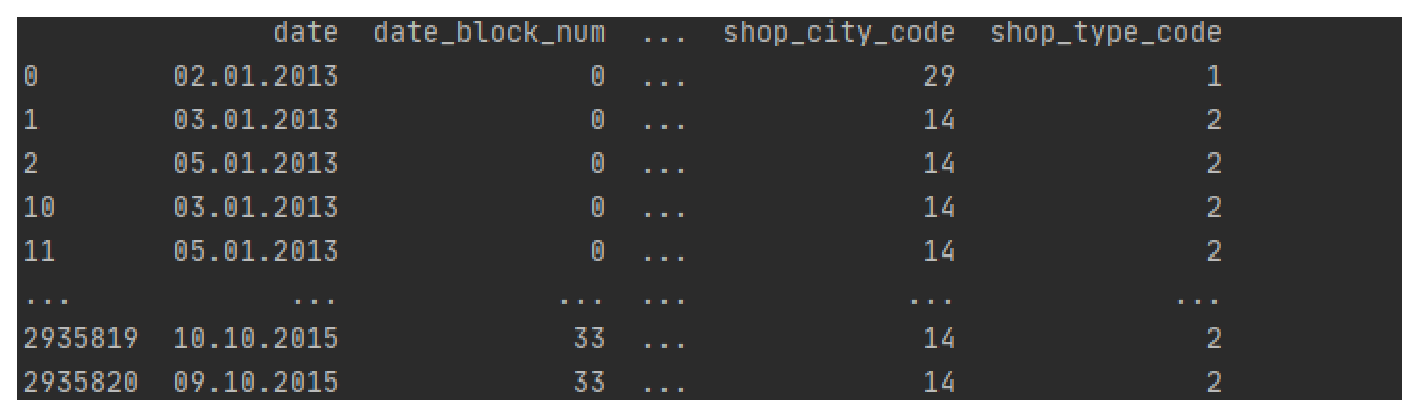
\includegraphics[width=0.88\textwidth]{logos/normal.eps}
%     \vspace{0.4em}
%     \caption{Normal Opreation}
%   \end{minipage}
% \end{figure}

\end{slide}

% \begin{slide}{Characteristics Of  The Processing}
%   \begin{itemize}
%     \item use historical sales data to predict future sales.\\
%     Using the historical sales data as the characteristics of the model, \\
%     this month's sales results as labels to build a model for regression analysis.
%     % \item From the ‘Dates’ field, we extracted the Day, the Month, the
%     %  Year, the Hour, the Minute, the Weekday, and the number of days 
%     %  since the first day in the data.
  
%     % \item From the ‘Address’ field we extracted if the incident has taken
%     %  place in a crossroad or on a building block.
%   \end{itemize}
%   \begin{figure}[htbp]
%     \centering
%     \begin{minipage}[t]{0.48\textwidth}
%       \centering
%       \centerline{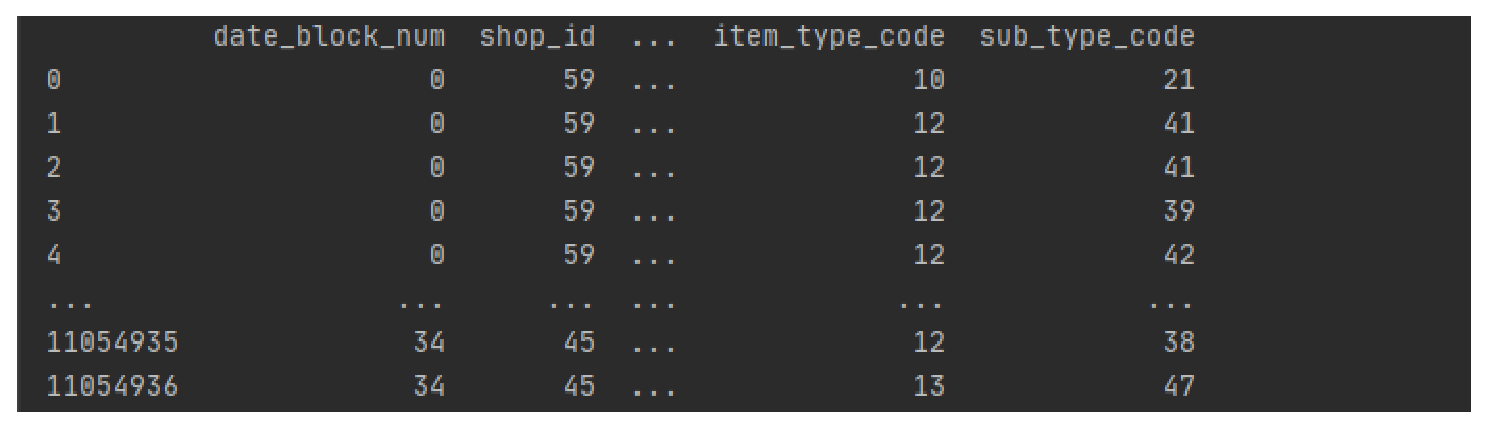
\includegraphics[width=0.88\textwidth]{logos/tezheng.eps}}
%       \vspace{-1.0em}
%       \caption{Fusion Feature}
%     \end{minipage}
%     % \begin{minipage}[t]{0.48\textwidth}
%     %   \centering
%     %   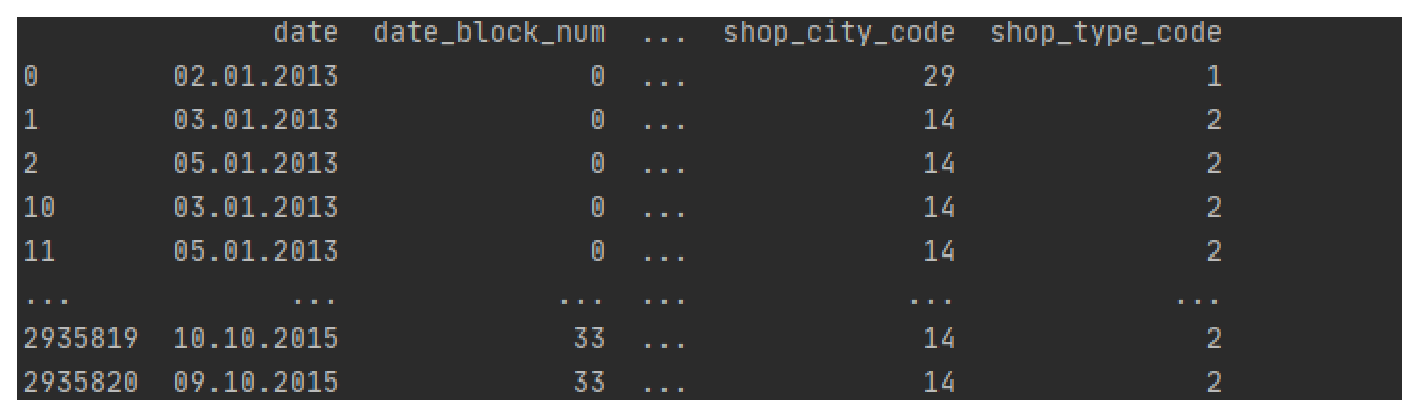
\includegraphics[width=0.88\textwidth]{logos/normal.eps}
%     %   \vspace{0.4em}
%     %   \caption{Normal Opreation}
%     % \end{minipage}
%   \end{figure}
%   \end{slide}




% \section{Model Adopted}

% %%
% %%============================================================================================

% %%
% %%==============================================================================================
% \begin{slide}{LightGBM Model}
%   This project uses lightGBM model for training.\\
%   LightGBM is a fast, distributed, high-performance gradient enhancement framework
%    based on decision tree algorithms.It supports category characteristics. \\
%    LightGBM supports category characteristics directly and natively by changing the decision rules
%   of the decision tree algorithm, without transformation.
%   \begin{figure}[htbp]
%     \centering
%     \begin{minipage}[t]{0.48\textwidth}
%       \centering
%       \centerline{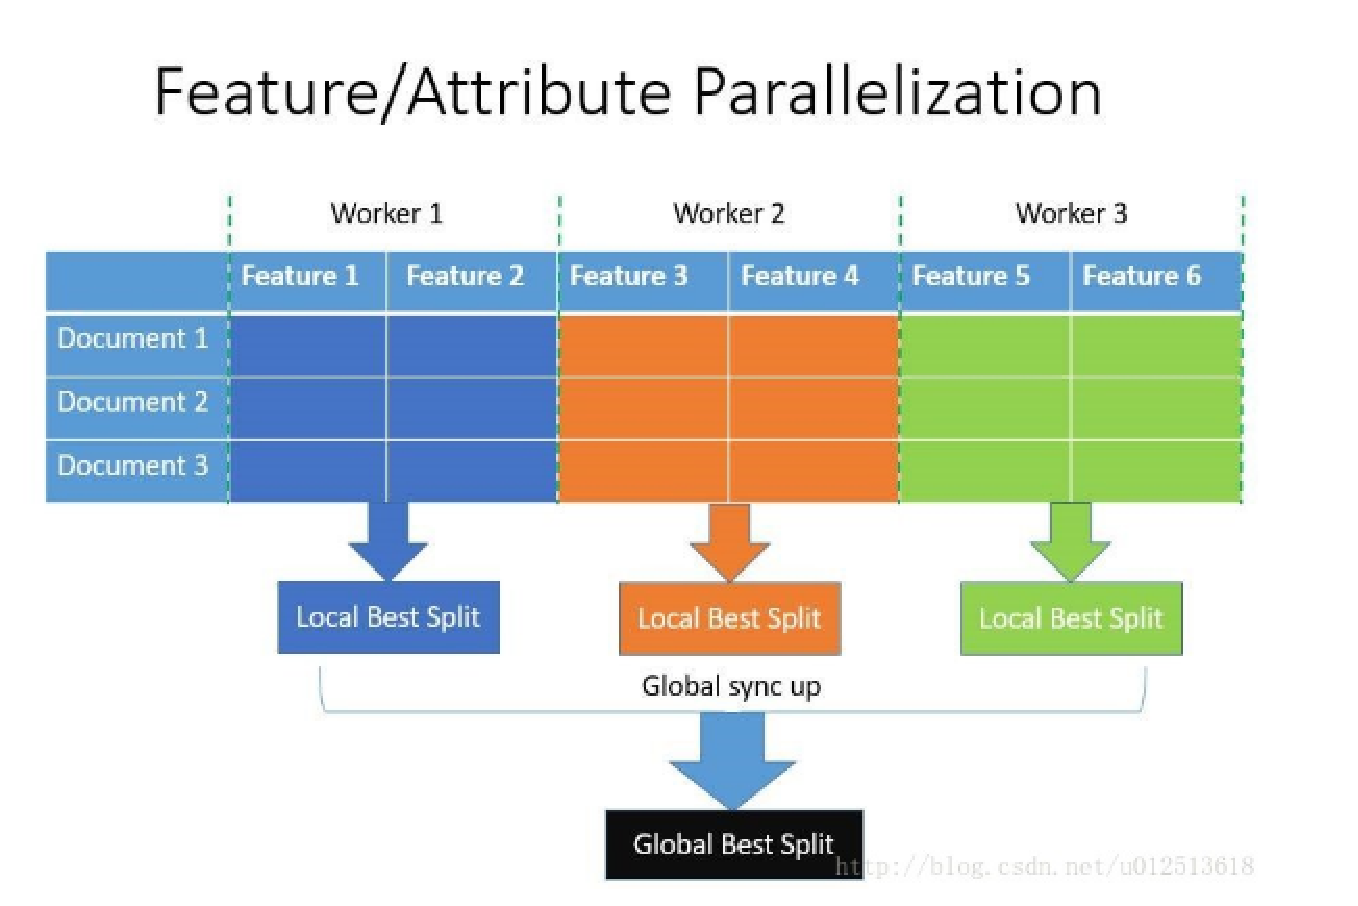
\includegraphics[width=0.88\textwidth]{logos/moxing.eps}}
%       \vspace{-1.0em}
%       \caption{Feature Parallelization}
%     \end{minipage}
%     % \begin{minipage}[t]{0.48\textwidth}
%     %   \centering
%     %   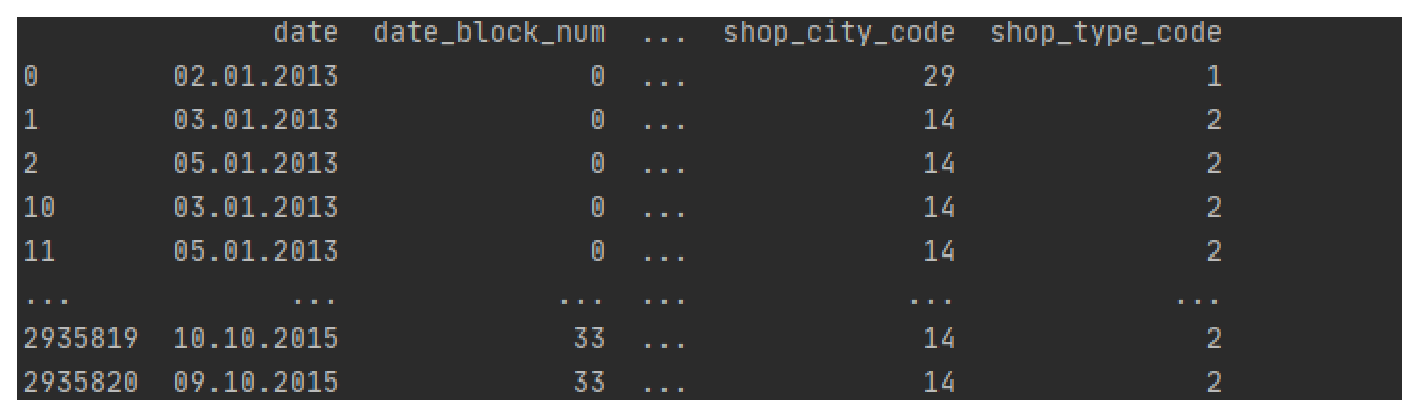
\includegraphics[width=0.88\textwidth]{logos/normal.eps}
%     %   \vspace{0.4em}
%     %   \caption{Normal Opreation}
%     % \end{minipage}
%   \end{figure}
% \end{slide}

%%
%%===============================================================================================


% \section{Summary}

% \begin{slide}{Project Summary}
%   From data analysis methods to feature engineering and prediction model construction,
%   a lot of time has been spent to study and comb.\\Through this project, I have learned a lot, 
%   including the effective aspects of problem cutting, code implementation of analysis algorithm, 
%   design of analysis process, etc.\\ which enables me to better grasp the thinking of data analysis on the whole.\\
%   In the process of predictive analysis, the theoretical and data support for feature analysis and model construction 
%   is not concise and powerful enough,which needs to be strengthened.
% \end{slide}
%%==========================================================================================
%%


% \section{Ideas Improvement}

% TODO: Contact Page

\end{document}

\endinput
